\newif\ifjournal
\journalfalse 

\ifjournal
	\documentclass[
						superscriptaddress, 																 amsmath, amssymb,
		 aps,  prb,  
										floatfix,
		linenumbers,
			]{revtex4-1}
\else
	\documentclass[
		superscriptaddress, 
		amsmath, 
		amssymb,
		aps,  
		prb, 
		notitlepage,
		floatfix,
	]{revtex4-1} 
\fi





\usepackage[utf8]{inputenc}   \usepackage[T1]{fontenc}
\usepackage{textcomp}             
\usepackage{bm}					\usepackage{enumerate}
\usepackage[hidelinks]{hyperref}    \usepackage[mathlines]{lineno}	\pdfoutput=1 					       
\usepackage{graphicx}			
\usepackage{multirow}
\usepackage{dcolumn}			\usepackage[usenames, dvipsnames]{colortbl} 
\usepackage[normalem]{ulem} 



\newcommand{\bket}[1]{\left<#1\right>}
\newcommand{\scprod}[2]{\left<#1|#2\right>}
\newcommand{\ket}[1]{\left|#1\right>}
\newcommand{\bra}[1]{\left<#1\right|}
\newcommand{\tr}[1]{\text{Tr}\left(#1\right)}
\newcommand{\kket}[1]{\left|\left|#1\right>\right>}
\newcommand{\bbra}[1]{\left<\left<#1\right|\right|}
\newcommand{\kb}[1]{\left|#1\right>\left<#1\right|}
\global\long\def\ketbra#1#2{\left|#1\vphantom{#2}\right\rangle \left\langle \vphantom{#1}#2\right|}
\newcommand{\bsz}{\text{\bf{\sigma_z}}}
\newcommand{\abs}[1]{\left|#1\right|}
\newcommand{\red}[1]{\colorbox{Apricot}{#1}}



\newcommand{\B}{\ket{\mathrm{B}}}
\newcommand{\G}{\ket{\mathrm{G}}}
\newcommand{\D}{\ket{\mathrm{D}}}

\newcommand{\m}[1]{\mathrm{\mathbf{#1}}}  \newcommand{\mh}[1]{
    \boldsymbol{ \hat{ \mathrm{ #1 } } }
} 




\begin{document}

\renewcommand{\figurename}{\textbf{Figure}}
\renewcommand{\tablename}{\textbf{Table}}

\title{Supplementary Information for:\\ ``To catch and reverse a quantum jump mid-flight''}

\author{Z.K. Minev}
 \email{zlatko.minev@aya.yale.edu | zlatko-minev.com}
 \affiliation{Department of Applied Physics, Yale University, New Haven, Connecticut 06511, USA}
  \author{S.O. Mundhada}
   \affiliation{Department of Applied Physics, Yale University, New Haven, Connecticut 06511, USA}
\author{S. Shankar}
   \affiliation{Department of Applied Physics, Yale University, New Haven, Connecticut 06511, USA}
\author{P. Reinhold}
   \affiliation{Department of Applied Physics, Yale University, New Haven, Connecticut 06511, USA}
\author{R. Guti\'errez-J\'auregui}
   \affiliation{The Dodd-Walls Centre for Photonic and Quantum Technologies, Department of Physics, University of Auckland, Private Bag 92019, Auckland, New Zealand}
\author{R.J. Schoelkopf}
   \affiliation{Department of Applied Physics, Yale University, New Haven, Connecticut 06511, USA}
\author{M. Mirrahimi}
	\affiliation{Yale Quantum Institute, Yale University, New Haven, Connecticut 06520, USA}
	\affiliation{QUANTIC team, INRIA de Paris, 2 Rue Simone Iff, 75012 Paris, France}
\author{H.J. Carmichael}
   \affiliation{The Dodd-Walls Centre for Photonic and Quantum Technologies, Department of Physics, University of Auckland, Private Bag 92019, Auckland, New Zealand}
\author{M.H. Devoret}
   \affiliation{Department of Applied Physics, Yale University, New Haven, Connecticut 06511, USA}

\date{\today}

\maketitle
\vspace{5em}
\tableofcontents
\clearpage






\onecolumngrid
\makeatletter
\makeatletter
\renewcommand{\fnum@figure}{\textbf{Supplementary Figure~\thefigure}}
\renewcommand{\fnum@table}{\textbf{Supplementary Table~\thetable}}
\makeatother

\renewcommand{\thefigure}{S\arabic{figure}}
\renewcommand{\thetable}{S\arabic{table}}
\setcounter{figure}{0}







\section{Experimental characterization of the system}

\begin{figure}[!b]
\begin{centering}
\ifjournal
	\includegraphics[width=140mm]{../main/img/supplementary/time-resolved-tomo-D.pdf}
\else
	\includegraphics[width=140mm]{time-resolved-tomo-D.pdf}
\fi
\caption{\label{fig:time-resolved-tomo-D}
\textbf{Control experiment: time-resolved tomogram of the free evolution of a DG superposition.}
The atom is prepared in $\frac{1}{\sqrt{2}} \left( \D - \G \right)$ and tomography is performed after a varied delay.  Dots: reconstructed conditional GD tomogram ($X_\mathrm{DG},Y_\mathrm{DG},$ and $Z_\mathrm{DG}$) and population in DG manifold,  $N$ (see Methods). Solid lines: theoretical fits.
}
\end{centering}
\end{figure}

\textit{Hamiltonian of the device.}
The two-transmon, single-readout-cavity system is well described, in the low-excitation manifold, by the approximate dispersive Hamiltonian\cite{Nigg2012}${}^{,}$\footnote{Z. K. Minev \textit{et al.}, Energy-participation approach to the design of quantum Josephson circuits, in prep.}: \begin{eqnarray}
\hat{H}/\hbar&=& \omega_{\mathrm{B}}\hat{b}^{\dagger}\hat{b}-\frac{1}{2}\alpha_{\mathrm{B}}\hat{b}^{\dagger2}\hat{b}^{2}+\omega_{\mathrm{D}}\hat{d}^{\dagger}\hat{d}-\frac{1}{2}\alpha_{\mathrm{D}}\hat{d}^{\dagger2}\hat{d}^{2}-\chi_{\mathrm{DB}}\hat{b}^{\dagger}\hat{b}\hat{d}^{\dagger}\hat{d}\label{eq:Hamiltonian-of-sys}\\
 &&+\left(\omega_{\mathrm{C}}+\chi_{\mathrm{B}}\hat{b}^{\dagger}\hat{b}+\chi_{\mathrm{D}}\hat{d}^{\dagger}\hat{d}\right)\hat{c}^{\dagger}\hat{c}\,,\nonumber
\end{eqnarray}
where $\omega_{\mathrm{C}}$, $\omega_{\mathrm{B}}$ and $\omega_{\mathrm{D}}$
are the cavity, bright, and dark qubit transition frequencies, $\hat{c}$,
$\hat{b}$ and $\hat{d}$ are the associated ladder operators, and
$\alpha$ and $\chi$ are the modal anharmonicities and dispersive
shifts, respectively. \footnote{
For related work on  three-level superconducting systems, see Refs.~\onlinecite{Gambetta2011-Purcell, Srinivasan2011, Diniz2013, Dumur2015, Roy2017-3qubits, Zhang2017}.}
The states $\ket{\mathrm{B}}$ and $\ket{\mathrm{D}}$
correspond to one excitation in the bright ($\hat{b}^{\dagger}\ket 0$)
and dark ($\hat{d}^{\dagger}\ket 0$) modes, respectively.
The measured parameters of the device and the mode coherences are summarized in Table~\ref{tab:system-params}.




\begin{table}
\begin{centering}
\renewcommand*\arraystretch{1.5}\begin{tabular}{rl|rl|rl}
\multicolumn{2}{c|}{\textbf{Readout cavity}} & \multicolumn{2}{c|}{\textbf{BG transition}} & \multicolumn{2}{c}{\textbf{DG transition}}\tabularnewline
\hline
\hline
\multicolumn{6}{c}{\textbf{\rule{0pt}{5ex}Mode frequencies and non-linear parameters}}\tabularnewline
\hline
\textbf{\rule{0pt}{4ex}}$\mkern11mu\omega_{\mathrm{C}}/2\pi=$ & $8979.640\text{\,MHz}$ & ~$\omega_{\mathrm{BG}}/2\pi=$ & $5570.349\text{\,MHz}$ & ~$\omega_{\mathrm{DG}}/2\pi=$ & $4845.255\text{\,MHz}$\tabularnewline
 &  & $\chi_{\mathrm{B}}/2\pi=$ & $-5.08\pm0.2\,\mathrm{MHz}$~ & $\chi_{\mathrm{D}}/2\pi=$ & $-0.33\pm0.08\,\mathrm{MHz}$\tabularnewline
 &  & $\alpha_{\mathrm{B}}/2\pi=$ & $195\pm2\,\mathrm{MHz}$ & $\alpha_{\mathrm{D}}/2\pi=$ & $152\pm2\,\mathrm{MHz}$\tabularnewline
 &  & \multicolumn{4}{c}{$\chi_{\mathrm{DB}}/2\pi=61\pm2\,\mathrm{MHz}$}\tabularnewline
\multicolumn{6}{c}{\textbf{\rule{0pt}{5ex}Coherence related parameters}}\tabularnewline
\hline
\textbf{\rule{0pt}{5ex}}$\mkern12mu\kappa/2\pi$= & $3.62\pm0.05\,\mathrm{MHz}\mkern12mu$ & $T_{\mathrm{1}}^{\mathrm{B}}=$ & $28\pm2\,\mathrm{\mu s}$ & $T_{\mathrm{1}}^{\mathrm{D}}=$ & $116\pm5\,\mathrm{\mu s}$\tabularnewline
$\eta=$ & $0.33\pm0.03$ & $T_{\mathrm{2\mathrm{R}}}^{\mathrm{B}}=$ & $18\pm1\,\mathrm{\mu s}$ & $T_{\mathrm{2\mathrm{R}}}^{\mathrm{D}}=$ & $120\pm5\,\mathrm{\mu s}$\tabularnewline
$T_{\mathrm{int}}=$ & $260.0\,\mathrm{ns}$ & $T_{\mathrm{2\mathrm{E}}}^{\mathrm{B}}=$ & $25\pm2\,\mathrm{\mu s}$ & $T_{\mathrm{2\mathrm{E}}}^{\mathrm{D}}=$ & $162\pm6\,\mathrm{\mu s}$\tabularnewline
$n_{\mathrm{th}}^{\mathrm{C}}\le$ & $0.0017\pm0.0002$ & $n_{\mathrm{th}}^{\mathrm{B}}\le$ & $0.01\pm0.005$ & $n_{\mathrm{th}}^{\mathrm{D}}\le$ & $0.05\pm0.01$\tabularnewline
\multicolumn{6}{c}{\textbf{\rule{0pt}{5ex}Drive amplitude and detuning parameters}}\tabularnewline
\hline
\textbf{\rule{0pt}{5ex}}$\mkern12mu\bar{n}=$ & $5.0\pm0.2\mkern12mu$ & ~$\Omega_{\mathrm{B}0}/2\pi=$ & $1.2\pm0.01\,\mathrm{MHz}$ & ~$\Omega_{\mathrm{DG}}/2\pi=$ & $20\pm2\,\mathrm{kHz}$\tabularnewline
 &  & ~$\Omega_{\mathrm{B}1}/2\pi=$ & $600\pm10\,\mathrm{kHz}$ &  & \tabularnewline
$\Delta_{\mathrm{R}}=$ & $\chi_{\mathrm{B}}$ & ~$\Delta_{\mathrm{B}1}/2\pi=$ & $-30.0\,\text{MHz}$ & ~$\Delta_{\mathrm{DG}}/2\pi=$ & $-275.0\,\text{kHz}$\tabularnewline
\end{tabular}
\par\end{centering}
\caption{\textbf{\label{tab:system-params}Compilation of the experimental
parameters.}}
\end{table}

\vspace{10em}

\begin{figure}[hbt]
\begin{centering}
\ifjournal
	\includegraphics[width=88mm]{../main/img/supplementary/T1-vs-nbar.pdf}
\else
	\includegraphics[width=88mm]{T1-vs-nbar.pdf}
\fi
\caption{\label{fig:T1-vs-nbar}
\textbf{Measurement-induced energy relaxation $T_1(\bar{n})$.}
Energy relaxation rate ($T_1^{-1}$) of $\B$ (blue dots) and $\D$ (red dots) as a function of $\bar{n}$, measured with the following protocol:
after the atom is prepared in either $\B$ or $\D$, the readout tone ($\mathrm R$) is turned on for duration $t_\mathrm{read}$ with amplitude $\bar{n}$ (corresponding to the number of steady-state photons in the readout cavity when excited on resonance), whereafter the population of the initial state is measured.
As in all other experiments, the readout drive is applied at the $\B$ cavity frequency ($\omega_\mathrm{C}-\chi_\mathrm{B}$).
The relaxation rates are extracted from exponential fits of the population decay as a function of $t_\mathrm{read}$, from $1.3\times10^7$ experimental realizations.
The solids lines are guides to the eye:
blue line indicates the rapid degradation of $T_1^\mathrm{B}$ as a function of the readout strength, while the red line indicates the nearly constants $T_1^\mathrm{D}$ of the protected dark level.
}
\end{centering}
\end{figure}


\textit{DG coherence \& tomography control.}
In Fig.~\ref{fig:time-resolved-tomo-D}, we show the results of a control experiment where we verified the Ramsey coherence ($T_\mathrm{2R}^\mathrm{D}$) and energy relaxation ($T_\mathrm{1}^\mathrm{D}$) times of the DG transition with our tomography method.
Solid lines are fitted theoretical curves for the free evolution of the prepared initial state $\frac{1}{\sqrt{2}} \left( \D - \G \right)$.
The $T_\mathrm{2R}^\mathrm{D} = 119.2\,\mathrm{\mu s}$ value gained from the simultaneous fit of $X_\mathrm{DG}(t)$ and $Y_\mathrm{DG}(t)$  matches the lifetime independently obtained from a standard $T_\mathrm{2R}$ measurement. Similarly, the  value of  $T_\mathrm{1}^\mathrm{D} = 115.4\,\mathrm{\mu s}$ extracted from an exponential fit of  $Z_\mathrm{DG}(t)$ matches the value obtained from a standard $T_\mathrm{1}$ measurement. We note that our tomography procedure is well calibrated and skew-free, as evident in the zero steady-state values of $X_\mathrm{DG}$ and $Y_\mathrm{DG}$. The steady state $Z_\mathrm{DG}$ corresponds to the  thermal population of the dark state $n_{\mathrm{th}}^{\mathrm{D}}$. It has recently been shown that residual thermal populations in cQED systems can be significantly reduced by properly thermalizing the input-output lines.\cite{Yeh2017Atten,Wang2019-cav-atten}


\textit{Measurement-induced energy relaxation $T_1(\bar{n})$.} Figure~\ref{fig:T1-vs-nbar} shows a characterization of the parasitic measurement-induced energy relaxation  of $\B$ and $\D$.
As is the case in standard cQED systems\cite{Slichter2012, Slichter2016-T1vsNbar, Sank2016-T1vsNbar}, the $\B$ level shows strong $T_1$ degradation\cite{Boissonneault2008, Boissonneault2009-Photon-induced-relax,Verney2018,Lescanne2018} as a function of the readout drive strength $\bar{n}$.
However, the lifetime of the dark state ($\D$) is protected, and remains largely unaffected even at large drive strengths ($\bar{n}\approx50$).





\section{Quantum trajectory theory}
\label{sec:quantum-traj-theory}

\subsection{Fluorescence monitored by photon counts}
\label{sec:fluorescence_monitored_by_photon_counts}
\subsubsection{Coherent Bright drive} 
The experiments with trapped ions \cite{Nagourney1986,Sauter1986,Bergquist1986} monitor intermittent fluorescence from the bright state $|{\rm B}\rangle$ to track jumps between $|{\rm G}\rangle$ and $|{\rm D}\rangle$.\cite{Cook1985} In the simplest three-level scheme,\cite{Bergquist1986} and using coherent radiation to excite both  transitions, the master equation for the reduced density operator $\rho$  of the three-level system, written in the interaction picture, is
\begin{equation}
\frac{\mathrm{d}\rho}{\mathrm{d}t}=(i\hbar)^{-1}[\hat H_{\rm drive},\rho]+\gamma_{\rm B}{\cal D}\left[|{\rm G}\rangle\langle{\rm B}|\right]\rho+\gamma_{\rm D}{\cal D}\left[|{\rm G}\rangle\langle{\rm D}|\right]\rho,
\end{equation}
where ${\cal D}[\hat \xi]\mkern3mu\cdot=\hat \xi\cdot \xi^\dagger-\frac12\{\hat \xi^\dagger\hat \xi,\cdot\mkern3mu\}$ denotes the Lindblad superoperator, $\gamma_{\rm B}$ and $\gamma_{\rm D}$ are radiative decay rates, and
\begin{equation}
\hat H_{\rm drive}=i\hbar\frac{\Omega_{\rm BG}}2\big(|{\rm B}\rangle\langle {\rm G}|-|{\rm G}\rangle\langle{\rm B}|\big)+i\hbar\frac{\Omega_{\rm DG}}2\big(|{\rm D}\rangle\langle{\rm G}|-|{\rm G}\rangle\langle{\rm D}|\big),
\label{eqn:drive_coherent_fluorescence}
\end{equation}
with $\Omega_{\rm BG}$ and $\Omega_{\rm DG}$ the Rabi drives. The quantum trajectory description\cite{Carmichael1993,Dalibard1992-original-traj,Dum1992} unravels $\rho$ into an ensemble of pure states whose ket vectors evolve along stochastic paths conditioned on the clicks of imaginary photon detectors that monitor fluorescence from $|{\rm B}\rangle$ (and much less frequently from $|{\rm D}\rangle$). In recognition of each click the ket vector is reset to $|{\rm G}\rangle$, while otherwise it follows a deterministic evolution as a coherent superposition,
\begin{equation}
|\psi(\Delta t_{\rm catch})\rangle=C_{\rm G}(\Delta t_{\rm catch})|{\rm G}\rangle+C_{\rm B}(\Delta t_{\rm catch})|{\rm B}\rangle+C_{\rm D}(\Delta t_{\rm catch})|{\rm D}\rangle,
\label{eqn:GBD-ket}
\end{equation}
where $C_{\rm G}(0)=1$, $C_{\rm B}(0)=C_{\rm D}(0)=0$, with $\Delta t_{\rm catch}=0$ marking the time of the last click reset, and
\begin{equation}
i\hbar\frac{\mathrm{d}|\psi\rangle}{\mathrm{d}\Delta t_{\rm catch}}=\left(\mkern-2mu \hat H_{\rm drive}-i\hbar\frac{\gamma_{\rm B}}2|{\rm B}\rangle\langle{\rm B}|-i\hbar\frac{\gamma_{\rm D}}2|{\rm D}\rangle\langle{\rm D}|\right)\mkern-3mu|\psi\rangle.
\label{eqn:between_click_equation}
\end{equation}
The norm of the ket $|\psi(\Delta t_{\rm catch})\rangle$ is not preserved, but rather gives the probability that the evolution will continue, with no interruption by further clicks, up to time $\Delta t_{\rm catch}$; clearly it must decay with this probability to zero.
If we then define
\begin{equation}
W_{\rm DG}(\Delta t_{\rm catch})\equiv\frac{C_{\rm D}(\Delta t_{\rm catch})}{C_{\rm G}(\Delta t_{\rm catch})},
\label{eqn:W_DG_definition}
\end{equation}
the \textit{normalized} ket vector in the GD-subspace has Bloch vector components
\begin{eqnarray}
{\rm Z}_{\rm GD}(\Delta t_{\rm catch})&=&\frac{W_{\rm DG}(\Delta t_{\rm catch})-W_{\rm DG}^{-1}(\Delta t_{\rm catch})}{W_{\rm DG}(\Delta t_{\rm catch})+W_{\rm DG}^{-1}(\Delta t_{\rm catch})},
\label{eqn:Z}\\
\noalign{\vskip4pt}
{\rm X}_{\rm GD}(\Delta t_{\rm catch})&=&\frac2{W_{\rm DG}(\Delta t_{\rm catch})+W_{\rm DG}^{-1}(\Delta t_{\rm catch})},
\label{eqn:X}\\
\noalign{\vskip6pt}
{\rm Y}_{\rm GD}(\Delta t_{\rm catch})&=&0,
\label{eqn:Y}
\end{eqnarray}
where, using Eqs.~(\ref{eqn:GBD-ket}) and (\ref{eqn:between_click_equation}),
\begin{equation}
\frac{d}{d\Delta t_{\rm catch}}\mkern-2mu\left(
\begin{matrix}
C_{\rm G}\\
C_{\rm B}\\
C_{\rm D}
\end{matrix}
\right)=\frac12\left(
\begin{matrix}
0&-\Omega_{\rm BG}&-\Omega_{\rm DG}\\
\Omega_{\rm BG}&-\gamma_{\rm B}&0\\
\Omega_{\rm DG}&0&-\gamma_{\rm D}\\
\end{matrix}
\right)\mkern-4mu\left(
\begin{matrix}
C_{\rm G}\\
C_{\rm B}\\
C_{\rm D}
\end{matrix}
\right).
\label{eqn:3x3_system}
\end{equation}
In general this $3\times3$ system does not have a closed solution in simple form, although there is a particularly simple solution under conditions  that produce intermittent fluorescence, i.e., rare jumps from $|{\rm G}\rangle$ to $|{\rm D}\rangle$ (``shelving'' in the dark state \cite{Nagourney1986}) interspersed as intervals of fluorescence ``off'' in a background of fluorescence ``on''. The conditions follow naturally if $|{\rm D}\rangle$ is a metastable state,\cite{Nagourney1986,Sauter1986,Bergquist1986,Macieszczak2016} whose lifetime $\gamma_{\rm D}^{-1}$ is extremely long on the scale of the mean time  between photon detector clicks for a weak $\Omega_{\rm BG}$ Rabi drive,
\begin{equation}
\Gamma_\mathrm{BG}^{-1} = \left(\frac{\Omega_{\rm BG}^2}{\gamma_{\rm B}}\right)^{-1}\;. 
\label{eq:GammaBG}
\end{equation}
Thus, for $(\Omega_{\rm DG},\gamma_{\rm D})\ll\Omega_{\rm BG}^2/\gamma_{\rm B}\ll\gamma_{\rm B}$, Eq.~(\ref{eqn:3x3_system}) yields the equation of motion
\begin{equation}
\frac{\mathrm{d}W_{\rm DG}}{\mathrm{d}\Delta t_{\rm catch}}=\frac{\Omega_{\rm BG}^2}{2\gamma_{\rm B}}W_{\rm DG}+\frac{\Omega_{\rm DG}}2,
\label{eqn:W_DG_equation_coherent}
\end{equation}
whose solution for the click reset initial condition, $W_{\rm DG}(0)=0$, is
\begin{equation}
W_{\rm DG}(\Delta t_{\rm catch})=\frac{\Omega_{\rm DG}}{\Omega^2_{\rm BG}/\gamma_{\rm B}}\left[\exp\left(\frac{\Omega^2_{\rm BG}}{2\gamma_{\rm B}}\Delta t_{\rm catch}\right)-1\right],
\label{eqn:W_DG_coherent}
\end{equation}
from which a long enough interval with no clicks gives $W_{\rm DG}(\Delta t_{\rm catch})\gg1$ and leads to the conclusion that the ket vector is $|{\rm D}\rangle$.
The time scale for the transition, $\Delta t_{\rm mid}$, is defined by $Z_\mathrm{GD}(\Delta t_{\rm mid})=0$, which corresponds to $W_{\rm DG}(\Delta t_{\rm mid})=1$.\cite{Porrati1987} 
Simply inverting Eq.~\eqref{eqn:W_DG_coherent} produces the formula
\begin{equation}
\Delta t_{\rm mid}=\left(\frac{\Omega^2_{\rm BG}}{2\gamma_{\rm B}}\right)^{-1}\ln\left(\frac{\Omega^2_{\rm BG}/\gamma_{\rm B}}{\Omega_{\rm DG}}+1\right),
\label{eqn:t_mid_coherent}
\end{equation}
but strong monitoring, $\Omega^2_{\rm BG}/\gamma_{\rm B}\gg\Omega_{\rm DG}$, allows the $-1$, in Eq.~(\ref{eqn:W_DG_coherent}), and $+1$, in Eq.~(\ref{eqn:t_mid_coherent}), to be dropped. Equations (\ref{eqn:Z})--(\ref{eqn:Y}), (\ref{eqn:W_DG_coherent}), and (\ref{eqn:t_mid_coherent}) then provide simple formulas for the continuous, deterministic, and coherent evolution of the quantum jump when completed:
\begin{eqnarray}
{\rm Z}_{\rm GD}(\Delta t_{\rm catch})&=&{\rm tanh}\left[\frac{\Omega^2_{\rm BG}}{2\gamma_B}(\Delta t_{\rm catch}-\Delta t_{\rm mid})\right],
\label{eqn:Z_approx}\\
\noalign{\vskip4pt}
{\rm X}_{\rm GD}(\Delta t_{\rm catch})&=&{\rm sech}\left[\frac{\Omega^2_{\rm BG}}{2\gamma_B}(\Delta t_{\rm catch}-\Delta t_{\rm mid})\right],
\label{eqn:X_approx}\\
\noalign{\vskip6pt}
{\rm Y}_{\rm GD}(\Delta t_{\rm catch})&=&0.
\label{eqn:Y_approx}
\end{eqnarray}
These formulas execute a perfect jump, ${\rm Z}_{\rm GD}(\infty)=1$, ${\rm X}_{\rm GD}(\infty)={\rm Y}_{\rm GD}(\infty)=0$. The ideal arises from the assumed strong monitoring, $\Omega_{\rm DG}\ll\Omega^2_{\rm BG}/\gamma_{\rm B}$. Departures from it can be transparently analyzed by adopting an incoherent Bright drive, see Sec.~\ref{sec:incoherent-B-drive}. 
An elegant analysis of the no-click evolution for arbitrary amplitude of the Dark Rabi drive can be found in Refs.~\onlinecite{Ruskov2007} and~\onlinecite{Ruskov2009-unpublished}. For an interesting connection to of the three-level intermittent dynamics to dynamical phase transitions, see Refs.~\onlinecite{Lesanovsky2013} and~\onlinecite{Garrahan2018}.



\textit{Application of the photon counting model to the experiment.} 
The photon-counting theory presented in this section  provides the background to the experiment along with a link to the original ion experiments.
It captures a core set of the ideas, even though the monitoring of $|\rm B\rangle$ implemented in the experiment is diffusive --- the opposite limit of the point-process description presented here, see Sec.~\ref{sec:Cavity-Monitor}. 
Nevertheless, the photon-counting theory even provides a quantitative first approximation of the experimental results. 
For definitiveness, consider the flight of the quantum jump shown in Fig.~3b.
The measured mid-flight time, $\Delta t_\mathrm{mid} = 3.95~\mathrm{\mu s}$, is predicted, in a first approximation, by Eq.~\eqref{eqn:t_mid_coherent}.
Using the (independently measured) values of the experimental parameters, summarized in Table~\ref{tab:system-params} (setting $\Omega_\mathrm{BG}$ equal to  $\Omega_\mathrm{B0} = 2\pi\times1.2$~MHz, the BG drive when the atom is not in $\ket{\rm B}$) and extracting the effective measurement rate of $|\rm B\rangle$, $\gamma_\mathrm{B} = 2\pi\times 9.0$~MHz (which follows from Eq.~\eqref{eq:GammaBG} where $\Gamma_\mathrm{BG} = 2\pi\times1.01$~MHz, the average click rate on the BG transition), Eq.~\eqref{eqn:t_mid_coherent} predicts $\Delta t_{\rm mid} \approx 4.3~\mathrm{\mu s}$ --- in fair agreement with the observed value $\Delta t_{\rm mid}  = 3.95~\mathrm{\mu s}$. 
The photodetection theory presented in in Sec.~\ref{sec:incoherent-B-drive} further improves the agreement. These calculations serve to generally illustrate the theory and ideas of the experiment; the quantitative comparison between theory and experiment is only presented in Sec.~\ref{sec:Comparison-theory-exp}.


\subsubsection{Incoherent Bright drive} 
\label{sec:incoherent-B-drive}
If the coherent Rabi drive $\Omega_{\rm BG}$ is replaced by an incoherent drive $\Gamma_{\rm BG}$, the master equation in the interaction picture becomes
\begin{equation}
\frac{\mathrm{d}\rho}{\mathrm{d}t}=(i\hbar)^{-1}[\hat H_{\rm drive},\rho]+\Gamma_{\rm BG}{\cal D}[|{\rm B}\rangle\langle{\rm G}|]\rho+(\gamma_{\rm B}+\Gamma_{\rm BG}){\cal D}[|{\rm G}\rangle\langle{\rm B}|]\rho+\gamma_{\rm D}{\cal D}[|{\rm G}\rangle\langle{\rm D}|]\rho,
\end{equation}
where
\begin{equation}
\hat H_{\rm drive}=i\hbar\frac{\Omega_{\rm DG}}2\big(|{\rm D}\rangle\langle{\rm G}|-|{\rm G}\rangle\langle{\rm D}|\big).
\end{equation}
The previous weak drive assumption, $\Omega_{\rm BG}^2/\gamma_{\rm B}\ll\gamma_{\rm B}$, is now carried over with the assumption $\Gamma_{\rm BG}\ll\gamma_{\rm B}$, which says that the time between clicks in fluorescence is essentially the same as the time separating photon absorptions from the incoherent drive, as absorption is rapidly followed by fluorescence ($\gamma_{\rm B}+\Gamma_{\rm BG}\gg\Gamma_{\rm BG}$). This brings a useful simplification, since, following each reset to $|{\rm G}\rangle$, the unnormalized ket evolves in the GD-subspace,
\begin{equation}
i\hbar\frac{\mathrm{d}|\psi\rangle}{\mathrm{d}\Delta t_{\rm catch}}=\left(\mkern-2mu H_{\rm drive}-i\hbar\frac{\Gamma_{\rm BG}}2|{\rm G}\rangle\langle{\rm G}|-i\hbar\frac{\gamma_{\rm D}}2|{\rm D}\rangle\langle{\rm D}|\right)\mkern-3mu|\psi\rangle,
\end{equation}
thus replacing Eqs.~(\ref{eqn:3x3_system}) and (\ref{eqn:W_DG_equation_coherent}) by the simpler $2\times2$ system
\begin{equation}
\frac{\mathrm{d}}{d\Delta t_{\rm catch}}\mkern-2mu\left(
\begin{matrix}
C_{\rm G}\\
C_{\rm D}
\end{matrix}
\right)=\frac12\left(
\begin{matrix}
-\Gamma_{\rm BG}&-\Omega_{\rm DG}\\

\Omega_{\rm DG}&-\gamma_{\rm D}\\
\end{matrix}
\right)\mkern-4mu\left(
\begin{matrix}
C_{\rm G}\\
C_{\rm D}
\end{matrix}
\right),
\end{equation}
and, if $\gamma_{\rm D}\ll\Gamma_{\rm BG}$, the equation of motion
\begin{equation}
\frac{dW_{\rm DG}}{\mathrm{d}\Delta t_{\rm catch}}=\frac{\Gamma_{\rm BG}}2W_{\rm DG}+\frac{\Omega_{\rm DG}}2(1+W_{\rm DG}^2),
\label{eqn:W_DG_equation_incoherent}
\end{equation}
with solution, for $W_{\rm DG}(0)=0$,
\begin{equation}
W_{\rm DG}(\Delta t_{\rm catch})=\frac{\exp\left[(V-V^{-1})\Omega_{\rm DG}\Delta t_{\rm catch}/2\right]-1}{V-V^{-1}\exp\left[(V-V^{-1})\Omega_{\rm DG}\Delta t_{\rm catch}/2\right]},
\label{eqn:W_DG_incoherent}
\end{equation}
where
\begin{equation}
V=\frac12\frac{\Gamma_{\rm BG}}{\Omega_{\rm DG}}+\sqrt{\frac14\left(\frac{\Gamma_{\rm BG}}{\Omega_{\rm DG}}\right)^2-1}.
\end{equation}
In Ref.~\onlinecite{Ruskov2007}, a general form of the Bloch vector equations for arbitrary amplitude of the Rabi drive was found.
Inversion of the condition $W_{\rm DG}(\Delta  t_{\rm mid})=1$ gives the characteristic time scale
\begin{equation}
\Delta t_{\rm mid}=2\left[(V-V^{-1})\Omega_{\rm DG}\right]^{-1}\ln\left(\frac{V+1}{V^{-1}+1}\right).
\label{eqn:t_mid_incoherent}
\end{equation}
Equations (\ref{eqn:W_DG_incoherent})--(\ref{eqn:t_mid_incoherent}) replace Eqs.~(\ref{eqn:W_DG_coherent}) and (\ref{eqn:t_mid_coherent}); although, under strong monitoring ($\Gamma_{\rm BG}\gg\Omega_{\rm DG}$), they revert to these results with the substitution $\Omega_{\rm BG}^2/2\gamma_{\rm B}\to\Gamma_{\rm BG}/2$, recovering Eqs.~(\ref{eqn:Z})--(\ref{eqn:Y}) with the same substitution. More generally, $W_{\rm DG}(\Delta t_{\rm catch})$ goes to infinity at finite $\Delta t_{\rm catch}$, changes sign, and returns  from infinity to settle on the steady value $W_{\rm DG}(\infty)=-V$. The singular behavior marks a trajectory passing through the north pole of Bloch sphere. It yields the long-time solution
\begin{eqnarray}
{\rm Z}_{\rm GD}(\infty)=\sqrt{1-4\left(\frac{\Omega_{\rm DG}}{\Gamma_{\rm BG}}\right)^2},\qquad
{\rm X}_{\rm GD}(\infty)=-2\frac{\Omega_{\rm DG}}{\Gamma_{\rm BG}},\qquad
{\rm Y}_{\rm GD}(\infty)=0,
\label{eq:XYZ_GD-inf}
\end{eqnarray}
in contrast to the perfect jump of Eqs.~(\ref{eqn:Z_approx})--(\ref{eqn:Y_approx}).

\subsubsection{Dark drive off}
Turing the Dark drive off shortly after a click reset demonstrates the connection between the flight of a quantum jump and a projective measurement. From the point of view of the trajectory equations, the only change is the setting of $\Omega_{\rm DG}$ to zero at time $\Delta t_{\rm on}$ on the right-hand side of Eqs.~(\ref{eqn:W_DG_equation_coherent}) and (\ref{eqn:W_DG_equation_incoherent}). Subsequently, $W_{\rm DG}(\Delta t_{\rm catch})$ continues its exponential growth at rate $\Omega_{\rm BG}^2/2\gamma_B$ [Eq.~(\ref{eqn:W_DG_equation_coherent})] or $\Gamma_{\rm BG}/2$ [Eq.~(\ref{eqn:W_DG_equation_incoherent})]. Equations (\ref{eqn:Z})--(\ref{eqn:Y})   for the GD Bloch components still hold, 
but now with
\begin{equation}
\Delta t_{\rm mid}=\left(\frac{\Omega_{\rm BG}^2}{2\gamma_B},\frac{\Gamma_{\rm BG}}2\right)^{-1}\ln\big[W_{\rm DG}^{ -2}(\Delta t_{\rm on})\big]\,,
\end{equation}
which can provide an estimate of $\Delta t'_\mathrm{mid}$, specifying the time at which $Z_\mathrm{GD} = 0$.

The evolution during $\Delta t_\mathrm{off}$, in the absence of $\Omega_\mathrm{DG}$, in effect realizes a projective measurement of whether the state of the atom is $|{\rm G}\rangle$ or $|{\rm D}\rangle$, where the normalized state at $\Delta t_{\rm on}$ is
\begin{equation}
\frac{|\psi(\Delta t_{\rm on})\rangle}{\sqrt{{\cal N}(\Delta t_{\rm on})}}=\frac{C_{\rm G}(\Delta t_{\rm on})|{\rm G}\rangle+C_{\rm D}(\Delta t_{\rm on})|{\rm D}\rangle}{\sqrt{{\cal N}(\Delta t_{\rm on})}},
\label{eqn:initial_state}
\end{equation}
with ${\cal N}(\Delta t_{\rm on})=C_{\rm G}^2(\Delta t_{\rm on})+C_{\rm D}^2(\Delta t_{\rm on})$ the probability for the jump to reach $\Delta t_{\rm catch}=\Delta t_{\rm on}$ after a click reset to $|{\rm G}\rangle$ at $\Delta t_{\rm catch}=0$. The probability for the jump to continue to $\Delta t_{\rm catch}>\Delta t_{\rm on}$ (given $\Delta t_{\rm on}$ is reached) is then
\begin{equation}
\label{eq:completion-prob}
\frac{{\cal N}(\Delta t_{\rm catch})}{{\cal N}(\Delta t_{\rm on})}=\frac{C_{\rm D}^2(\Delta t_{\rm on})}{{\cal N}(\Delta t_{\rm on})}+\frac{C_{\rm G}^2(\Delta t_{\rm on})}{{\cal N}(\Delta t_{\rm on})}\exp\mkern-2mu\left[-\left(\frac{\Omega_{\rm BG}^2}{\gamma_{\rm B}},\Gamma_{\rm BG}\right)\mkern-2mu\Delta t_{\rm catch}\right].
\end{equation}

\subsubsection{Completed and aborted evolutions of the jump transition}
 In this simple model, the probability for the trajectory to complete --- for the measurement to yield the result $|{\rm D}\rangle$ --- is obtained in the limit $\Delta t_\mathrm{catch}\rightarrow \infty$, 
 and, as expected,  is equal to the probability to occupy the state $|{\rm D}\rangle$ at time $\Delta t_{\rm on}$; i.e., the completion probability is $P_\mathrm{D}(\Delta t_{\rm on}) = C_{\rm D}^2(\Delta t_{\rm on})/{{\rm Norm}(\Delta t_{\rm on})}$.
It is helpful to illustrate this idea with an example. Consider the catch experiment of Fig.~3b in the absence of the Dark Rabi drive, $\Omega_\mathrm{DG}$. From $Z_\mathrm{GD} $, we can  estimate that out of all the trajectories that pass though the $\Delta t_{\rm on}$ mark approximately $P_\mathrm{D}(\Delta t_{\rm on})= (1+Z_\mathrm{GD}(\Delta t_{\rm on}))/2 \approx 8\%$ fully complete without an interruption. On the other hand, for those that pass the $\Delta t'_\mathrm{mid}$ mark, approximately 50\%  complete. It follows from Eq.~\eqref{eq:completion-prob}, that the  probability of the evolution to complete increases the further along the trajectory is. 
Although some of the jump evolutions abort at random, importantly, every single jump evolution that completes, and is thus recorded as a jump,  follows \textit{not} a random but an identical path in Hilbert space, i.e., a deterministic one. This path (of \textit{any}  jump) is determined   by Eq.~\eqref{eqn:W_DG_incoherent}, or, in the simpler model, by  the Eqs.~\eqref{eqn:Z_approx}-\eqref{eqn:Y_approx} for the components of the GD Bloch vector.


\subsection{Bright state monitored by dispersive cavity readout}
\label{sec:Cavity-Monitor}
\subsubsection{Stochastic Schr\"odinger equation}
Monitoring the quantum jump through fluorescence photon counts provides a clean and simple way of analyzing the deterministic character of the evolution. It is prohibitively challenging for an experiment, though, as the time origin $\Delta t_{\rm catch}=0$ is set by the click reset to $|{\rm G}\rangle$, and in an ensemble of measurements, all resets must be aligned on the very last click before an interval of deterministic evolution (Eqs.~(\ref{eqn:Z})--(\ref{eqn:Y})) in order for $\Delta t_{\rm mid}$ to be aligned over the ensemble; low detection efficiency---on the order of $10^{-3}$ or less\cite{Nagourney1986,Sauter1986,Bergquist1986}---in the first ion experiments does not permit this. Monitoring through a dispersive cavity readout provides a robust way of aligning $\Delta t_{\rm catch}=0$, hence $\Delta t_{\rm mid}$, over an ensemble of measurements. Leaving aside imperfections (see below), the master equation in the interaction picture is
\begin{equation}
\frac{\mathrm{d}\rho}{\mathrm{d}t}=(i\hbar)^{-1}[\hat H_{\rm drive},\rho]+(i\hbar)^{-1}[\hat H_{\rm R},\rho]+\kappa{\cal D}[\hat c]\rho,
\end{equation}
with
\begin{equation}
\hat H_{\rm drive}=i\hbar\left[\frac{\Omega_{\rm BG}(t)}2|{\rm B}\rangle\langle {\rm G}|-\frac{\Omega_{\rm BG}^*(t)}2|{\rm G}\rangle\langle{\rm B}|\right]+i\hbar\frac{\Omega_{\rm DG}}2\big(|{\rm D}\rangle\langle{\rm G}|-|{\rm G}\rangle\langle{\rm D}|\big),
\end{equation}
and
\begin{equation}
\hat H_{\rm R}=-\hbar\Delta_{\rm R}\hat c^\dagger\hat c+i\hbar\frac{\kappa}2\sqrt{\bar n}(\hat c^\dagger-\hat c)+\hbar\big(\chi_{\rm B}|{\rm B}\rangle\langle{\rm B}|+\chi_{\rm D}|{\rm D}\rangle\langle{\rm D}|\big)\hat c^\dagger\hat c,
\end{equation}
where the bi-chromatic drive $\Omega_{\rm BG}(t)=\Omega_{{\rm B}0}+\Omega_{{\rm B}1}\exp(-i\Delta_{{\rm B}1}t)$ replaces the Rabi drive $\Omega_{\rm BG}$ of Eq.~(\ref{eqn:drive_coherent_fluorescence}), $\bar n$ is the mean photon number in the readout cavity when driven on resonance, and $\Delta_{\rm R}$ is the detuning of the probe from the unshifted cavity resonance; the bi-chromatic drive facilitates transitions in both directions between $|{\rm G}\rangle$ and $|{\rm B}\rangle$, given that the bright level shifts when the cavity fills with photons. The quantum  trajectory unraveling monitors the reflected probe with efficiency $\eta$ and accounts for residual photon loss through random jumps; thus, the stochastic Schr\"odinger equation combines a continuous evolution (heterodyne readout channel),
\begin{equation}
\mathrm{d}|\psi\rangle=\left[\frac1{i\hbar}\left(\hat H_{\rm drive}+\hat H_{\rm R}-i\hbar\frac\kappa2\hat c^\dagger\hat c\right)\mkern-3mu\mathrm{d}t+\sqrt\eta\sqrt{\kappa}\mathrm{d}\zeta^{*}\hat c\right]\mkern-3mu|\psi\rangle,
\label{eqn:SSE_continuous}
\end{equation}
where
\begin{equation}
\label{eq:heterodyne-current}
\mathrm{d}\zeta=\sqrt\eta\sqrt\kappa\frac{\langle\psi|\hat a |\psi\rangle}{\langle\psi|\psi\rangle}\mathrm{d}t+\mathrm{d}Z,
\end{equation}
$\mathrm{d}Z$  is a complex Wiener increment, obeying $\operatorname{E}\left[\mathrm{d}Z\right]=0$, $\operatorname{E}\left[\mathrm{d}Z^{2}\right]=0$, and~$\operatorname{Var}\left[\mathrm{d}Z\right]=\operatorname{E}\left[\mathrm{d}Z^{*}\mathrm{d}Z\right]=\mathrm{d}t$, with random jumps (photon loss),
\begin{equation}
|\psi\rangle\to\hat c|\psi\rangle\qquad\hbox{at rate}\qquad(1-\eta)\kappa\frac{\langle\psi|\hat c^\dagger\hat c|\psi\rangle}{\langle\psi|\psi\rangle}.
\end{equation}
The monitored output $\mathrm{d}\zeta$ is scaled---to units of (readout cavity photon number)${}^{1/2}$---and filtered to generate simulated quadratures $I_{\rm rec}$ and $Q_{\rm rec}$ of the measurement record:
\begin{eqnarray}
\label{eq:dI_rec}
\mathrm{d}I_{\rm rec}&=&-\frac{\kappa_{\rm filter}}2\left[I_{\rm rec}\mathrm{d}t-\left(\eta\frac\kappa2\right)^{-1/2}{\rm Re}(\mathrm{d}\zeta)\right],
\label{eqn:simulated_I_int}\\
\label{eq:dQ_rec}
\mathrm{d}Q_{\rm rec}&=&-\frac{\kappa_{\rm filter}}2\left[Q_{\rm rec}\mathrm{d}t-\left(\eta\frac\kappa2\right)^{-1/2}{\rm Im}(\mathrm{d}\zeta)\right],
\label{eqn:simulated_Q_int}
\end{eqnarray}
where $\kappa_{\rm filter}$ is the bandwidth of the experimental readout amplifier chain.

\subsubsection{Independently measured imperfections}
The stochastic Schr\"odinger equation is supplemented by spontaneous and thermal jumps on both the $|{\rm G}\rangle$ to $|{\rm B}\rangle$ and $|{\rm G}\rangle$ to $|{\rm D}\rangle$ transitions, and by pure dephasing of the ${\rm GB}$ and ${\rm GD}$ coherences. With these processes included, the term
\begin{equation}
-i\hbar\left\{\left[\frac{\gamma_{\rm B}}2(n_{\rm th}^{\rm B}+1)+\gamma_{\rm B}^\phi\right]\mkern-3mu|{\rm B}\rangle\langle{\rm B}|+\left[\frac{\gamma_{\rm D}}2(n_{\rm th}^{\rm D}+1)+\gamma_{\rm D}^\phi\right]\mkern-3mu|{\rm D}\rangle\langle{\rm D}|+\frac{\gamma_{\rm B}n_{\rm th}^{\rm B}+\gamma_{\rm D}n_{\rm th}^{\rm D}}2|{\rm G}\rangle\langle{\rm G}|\right\}\nonumber
\end{equation}
is added to the non-Hermitian Hamiltonian $\hat H_{\rm drive}+\hat H_{\rm R}-i\hbar(\kappa/2)\hat c^\dagger\hat c$ on the right-hand side of Eq.~(\ref{eqn:SSE_continuous}), and there are additional random jumps
\begin{eqnarray}
|\psi\rangle\to|{\rm G}\rangle&&\qquad\hbox{at rate}\qquad\gamma_{\rm B}(n_{\rm th}^{\rm B}+1)\frac{\langle\psi|{\rm B}\rangle\langle{\rm B}|\psi\rangle}{\langle\psi|\psi\rangle}+\gamma_{\rm D}(n_{\rm th}^{\rm D}+1)\frac{\langle\psi|{\rm D}\rangle\langle{\rm D}|\psi\rangle}{\langle\psi|\psi\rangle},\\
\noalign{\vskip4pt}
|\psi\rangle\to|{\rm B}\rangle&&\qquad\hbox{at rate}\qquad\gamma_{\rm B}n_{\rm th}^{\rm B}\frac{\langle\psi|{\rm G}\rangle\langle{\rm G}|\psi\rangle}{\langle\psi|\psi\rangle}+2\gamma_{\rm B}^{\phi}\frac{\langle\psi|{\rm B}\rangle\langle{\rm B}|\psi\rangle}{\langle\psi|\psi\rangle},\\
\noalign{\vskip4pt}
|\psi\rangle\to|{\rm D}\rangle&&\qquad\hbox{at rate}\qquad\gamma_{\rm D}n_{\rm th}^{\rm D}\frac{\langle\psi|{\rm G}\rangle\langle{\rm G}|\psi\rangle}{\langle\psi|\psi\rangle}+2\gamma_{\rm D}^{\phi}\frac{\langle\psi|{\rm D}\rangle\langle{\rm D}|\psi\rangle}{\langle\psi|\psi\rangle}.
\end{eqnarray}
The parameters $\gamma_{\rm B,D}$, $n_{\rm th}^{\rm B,D}$, and $\gamma_{\rm B,D}^\phi$ are mapped to the independently measured parameters $T_{\rm B,D}^1$, $n_{\rm th}^{\rm G,D}$, and $T_{2{\rm R}}^{\rm B,D}$ listed in Table \ref{fig:T1-vs-nbar} (see below).

\subsubsection{Leakage from the {\rm GBD}-manifold}
The three-state manifold, $|{\rm G}\rangle$, $|{\rm B}\rangle$, and $|{\rm D}\rangle$, is not strictly closed. Rare transitions to higher excited states of the two-transmon system may occur. This possibility is included with the addition of the further term
\begin{equation}
-i\hbar\left\{\frac{\gamma_{\rm FG}}2|{\rm G}\rangle\langle{\rm G}|+\frac{\gamma_{\rm FD}}2|{\rm D}\rangle\langle{\rm D}|+\frac{\gamma_{\rm GF}+\gamma_{\rm DF}}2|{\rm F}\rangle\langle{\rm F}|\right\}\nonumber
\end{equation}
to the non-Hermitian Hamiltonian, and the associated additional random jumps,
\begin{eqnarray}
|\psi\rangle\to|{\rm F}\rangle&&\qquad\hbox{at rate}\qquad\gamma_{\rm FG}\frac{\langle\psi|{\rm G}\rangle\langle{\rm G}|\psi\rangle}{\langle\psi|\psi\rangle}+\gamma_{\rm FD}\frac{\langle\psi|{\rm D}\rangle\langle{\rm D}|\psi\rangle}{\langle\psi|\psi\rangle},\\
\noalign{\vskip4pt}
|\psi\rangle\to|{\rm G}\rangle&&\qquad\hbox{at rate}\qquad\gamma_{\rm GF}\frac{\langle\psi|{\rm F}\rangle\langle{\rm F}|\psi\rangle}{\langle\psi|\psi\rangle},\\
\noalign{\vskip4pt}
|\psi\rangle\to|{\rm D}\rangle&&\qquad\hbox{at rate}\qquad\gamma_{\rm DF}\frac{\langle\psi|{\rm F}\rangle\langle{\rm F}|\psi\rangle}{\langle\psi|\psi\rangle},
\label{eqn:jumps_to_F}
\end{eqnarray}
where $|{\rm F}\rangle$ is a single catch-all higher excited state.







\section{Comparison between experiment and theory}
\label{sec:Comparison-theory-exp}


\subsection{Simulated data sets}
\textit{Independently measured parameters.}
The parameters used in the simulations are listed in Table~\ref{table:table2}. In most cases they are set to the value at the center of the range quoted in Table \ref{tab:system-params}, but with three exceptions: (i) $T_1^{\rm B}$ and $T_1^{\rm D}$ are set to lower values in response to the photon number dependence of the readout displayed in Fig.~\ref{fig:T1-vs-nbar}; (ii) $\Omega_{\rm DG}/2\pi$ is set higher, but still falls inside the experimental error bars, and (iii) $n_{\rm th}^{\rm C}=0$. Of the three exceptions, only $\Omega_{\rm DG}/2\pi$ has a noticeable effect on the comparison between simulated and experimental data sets.

\textit{Leakage from the {\rm GBD}-manifold.} Additional random jumps to state $|{\rm F}\rangle$ are governed by four parameters that are not independently measured; they serve as fitting parameters, required to bring the simulation into agreement with the asymptotic behavior of ${\rm Z}(\Delta t_{\rm catch})$, which, without leakage to $|{\rm F}\rangle$, settles  to a value higher than is measured in the experiment. The evolution of the ${\rm X}(\Delta t_{\rm catch})$ is largely unaffected by the assignment of these parameters, where any change that does occur can be offset by adjusting $\Omega_{\rm DG}/2\pi$ while staying within the experimental error bars.

\textit{Ensemble average.} Simulated data sets are computed as an ensemble average by sampling an ongoing Monte Carlo simulation, numerically implementing the model outlined in Eqs.~(\ref{eqn:SSE_continuous})--(\ref{eqn:jumps_to_F}). Quadratures $I_{\rm rec}$ and $Q_{\rm rec}$ are computed from Eqs.~(\ref{eqn:simulated_I_int}) and (\ref{eqn:simulated_Q_int}), digitized with integration time $T_{\rm int}=260\mkern2mu{\rm ns}$, and then, as in the experiment, a hysteric filter is used to locate ``click'' events ($\Delta t_{\rm catch}=0$) corresponding to an inferred change of state from $|{\rm B}\rangle$ to not-$|{\rm B}\rangle$. During the subsequent sampling interval ($\Delta t_{\rm catch}\geq0$), the four quantities
\begin{equation}
\big({\rm Z}_{\rm GD}^j,{\rm X}_{\rm GD}^j,{\rm Y}_{\rm GD}^j,{\rm P}_{\rm BB}^j\big)(\Delta t_{\rm catch})=\big({\rm Z}_{\rm GD}^{\rm rec},{\rm X}_{\rm GD}^{\rm rec},{\rm Y}_{\rm GD}^{\rm rec},{\rm P}_{\rm BB}^{\rm rec}\big)(t_j+\Delta t_{\rm catch}),
\end{equation}
with $t_j$ is the click time and
\begin{eqnarray}
{\rm Z}_{\rm GD}^{\rm rec}(t)&=&\frac{\langle{\rm D}|\psi(t)\rangle\langle\psi(t)|{\rm D}\rangle-\langle{\rm G}|\psi(t)\rangle\langle\psi(t)|{\rm G}\rangle}{\langle\psi(t)|\psi(t)\rangle},\label{eqn:correlated_Z_GD}\\
\noalign{\vskip4pt}
{\rm X}_{\rm GD}^{\rm rec}(t)+i{\rm Y}_{\rm GD}^{\rm rec}(t)&=&2\frac{\langle{\rm D}|\psi(t)\rangle\langle\psi(t)|{\rm G}\rangle}{\langle\psi(t)|\psi(t)\rangle},\label{eqn:correlated_X_GD&Y_GD}\\
\noalign{\vskip4pt}
{\rm P}_{\rm BB}^{\rm rec}(t)&=&\frac{\langle{\rm B}|\psi(t)\rangle\langle\psi(t)|{\rm B}\rangle}{\langle\psi(t)|\psi(t)\rangle},
\end{eqnarray}
are computed, and running sums of each are updated. The sample terminates when the measurement record indicates a change of state from not-$|{\rm B}\rangle$ back to $|{\rm B}\rangle$. Finally, for comparison with the experiment, Bloch vector components are recovered from the average over sample intervals via the formula
\begin{equation}
\big({\rm Z}_{\rm GD},{\rm X}_{\rm GD},{\rm Y}_{\rm GD}\big)(\Delta t_{\rm catch})=\frac{\sum_j^{N(\Delta t_{\rm catch})}\big({\rm Z}_{\rm GD}^j,{\rm X}_{\rm GD}^j,{\rm Y}_{\rm GD}^j\big)(\Delta t_{\rm catch})}{N(\Delta t_{\rm catch})-\sum_j^{N(\Delta t_{\rm catch})}P_{\rm BB}^j(\Delta t_{\rm catch})},
\label{eqn:ensemble_average}
\end{equation}
where $N(\Delta t_{\rm catch})$ is the number of sample intervals that extend up to, or beyond, the time $\Delta t_{\rm catch}$. The simulation and sampling procedure is illustrated in Fig.~\ref{fig:monte-carlo}, and a comparison between the experiment and the simulation is provided in Fig.~\ref{fig:simulation_vs_experiment}.


The simulated and measured Bloch vector components are fit with expressions motivated by Eqs.~\eqref{eqn:Z_approx}-\eqref{eqn:Y_approx} and~\eqref{eq:XYZ_GD-inf}, modified to account for the effect of non-idealities in the experiment, 
\begin{align}
\mathrm{Z}_{\text{GD}}(\Delta t_{\operatorname{catch}}) & =\ensuremath{a+b\tanh(\Delta t_{\operatorname{catch}}/\tau+c)},\\
\ensuremath{\mathrm{X}_{\text{GD}}(\Delta t_{\operatorname{catch}})} & =a'+b'\operatorname{sech}(\Delta t_{\operatorname{catch}}/\tau'+c')\,,\\
\mathrm{Y}_{\text{GD}}(\Delta t_{\operatorname{catch}}) & =0\,.
\end{align}
The fit parameters  ($a,a',b,b',c,c',\tau,\tau'$) for the simulated and experimental data shown in Fig.~\ref{fig:simulation_vs_experiment} are compared in Table~\ref{tab:Comparison-of-parameters}. 
As imposed by Eq.~\eqref{eq:XYZ_GD-inf}, in the absence of $\Omega_{\rm DG}$ (turned off at time $\Delta t_{\rm on}=2\mkern2mu\mu{\rm s}$) $a'$, the  offset of $\mathrm{X}_{\text{GD}}$,  is strictly enforced to be zero.
The extracted simulation and experiment parameters are found to agree at the percent level. 



 
\begin{table}[t]
\begin{tabular}{ r  c  l | r  c  l | r  c  l }
$\vphantom{\vbox{\vskip12pt}}\mkern40mu$&\textbf{Readout cavity}&$\mkern40mu$&$\mkern44mu$&\textbf{BG transition}&$\mkern44mu$&$\mkern44mu$&\textbf{DG transition}&$\mkern44mu$\\
\hline
\hline
\end{tabular}
\vskip12pt
\begin{tabular}{ r  c  l | r  c  l | r  c  l }
\multicolumn{9}{c}{$\vphantom{\vbox{\vskip10pt}}$\textbf{Non-linear parameters}\hfill}\\
\hline
&$\hphantom{\hbox{\hskip4.2cm}}\mkern-16mu$&&$\vphantom{\vbox{\vskip12pt}}\mkern32mu\chi_{\rm B}/2\pi$&$=$&$-5.08\mkern3mu{\rm MHz}\mkern32mu$&$\vphantom{\vbox{\vskip14pt}}\mkern30mu\chi_{\rm D}/2\pi$&$=$&$-0.33\mkern3mu{\rm MHz}\mkern30mu$\\
\end{tabular}
\vskip12pt
\begin{tabular}{ r  c  l | r  c  l | r  c  l }
\multicolumn{9}{c}{$\vphantom{\vbox{\vskip10pt}}$\textbf{Coherence related parameters}\hfill}\\
\hline
$\vphantom{\vbox{\vskip12pt}}\mkern46mu\kappa/2\pi$&$=$&$3.62\mkern3mu{\rm MHz}\mkern46mu$&$\mkern61muT_{1}^{\rm B}$&$=$&$15\mkern3mu\mu{\rm s}\mkern81mu$&$\mkern48muT_{1}^{\rm D}$&$=$&$105\mkern3mu\mu{\rm s}\mkern74mu$\\
$\vphantom{\vbox{\vskip12pt}}\eta$&$=$&$0.33$&$T_{2}^{\rm B}$&$=$&$18\mkern3mu\mu{\rm s}$&$T_{2}^{\rm D}$&$=$&$120\mkern3mu\mu{\rm s}$\\
$\vphantom{\vbox{\vskip12pt}}T_{\rm int}$&$=$&$260.0\mkern3mu{\rm ns}$ & &&&&&\\
$\vphantom{\vbox{\vskip12pt}}n_{\rm th}^{\rm C}$&$=$&$0$&$n_{\rm th}^{\rm B}$&$=$&$0.01$&$n_{\rm th}^{\rm D}$&$=$&$0.05$\\
\end{tabular}
\vskip12pt
\begin{tabular}{ r  c  l | r  c  l | r  c  l }
\multicolumn{9}{c}{$\vphantom{\vbox{\vskip10pt}}$\textbf{Drive amplitude and detuning parameters}\hfill}\\
\hline
$\vphantom{\vbox{\vskip12pt}}\mkern72mu\bar{n}$&$=$&$5.0\mkern40mu\mkern56mu$&$\Omega_{{\rm B}0}/2\pi$&$=$&$1.2\mkern3mu{\rm MHz}$&$\Omega_{\rm DG}/2\pi$&$=$&$21.6\mkern3mu{\rm kHz}$\\
$\vphantom{\vbox{\vskip12pt}}$&&&$\mkern20mu\Omega_{{\rm B}1}/2\pi$&$=$&$600\mkern3mu{\rm kHz}\mkern30mu$&&&\\
$\vphantom{\vbox{\vskip12pt}}\Delta_{\rm R}$&$=$&$\chi_{\rm B}$&$\mkern22mu\Delta_{{\rm B}1}/2\pi$&$=$&$-30.0\mkern3mu{\rm MHz}\mkern31mu$&$\mkern19mu\Delta_{\rm DG}/2\pi$&$=$&$-274.5\mkern3mu{\rm kHz}\mkern30mu$\\
\end{tabular}
\caption{\textbf{Compilation of the simulation parameters.}}
\label{table:table2}
\end{table}

\begin{figure}[t]
\begin{centering}
\vskip0.5cm
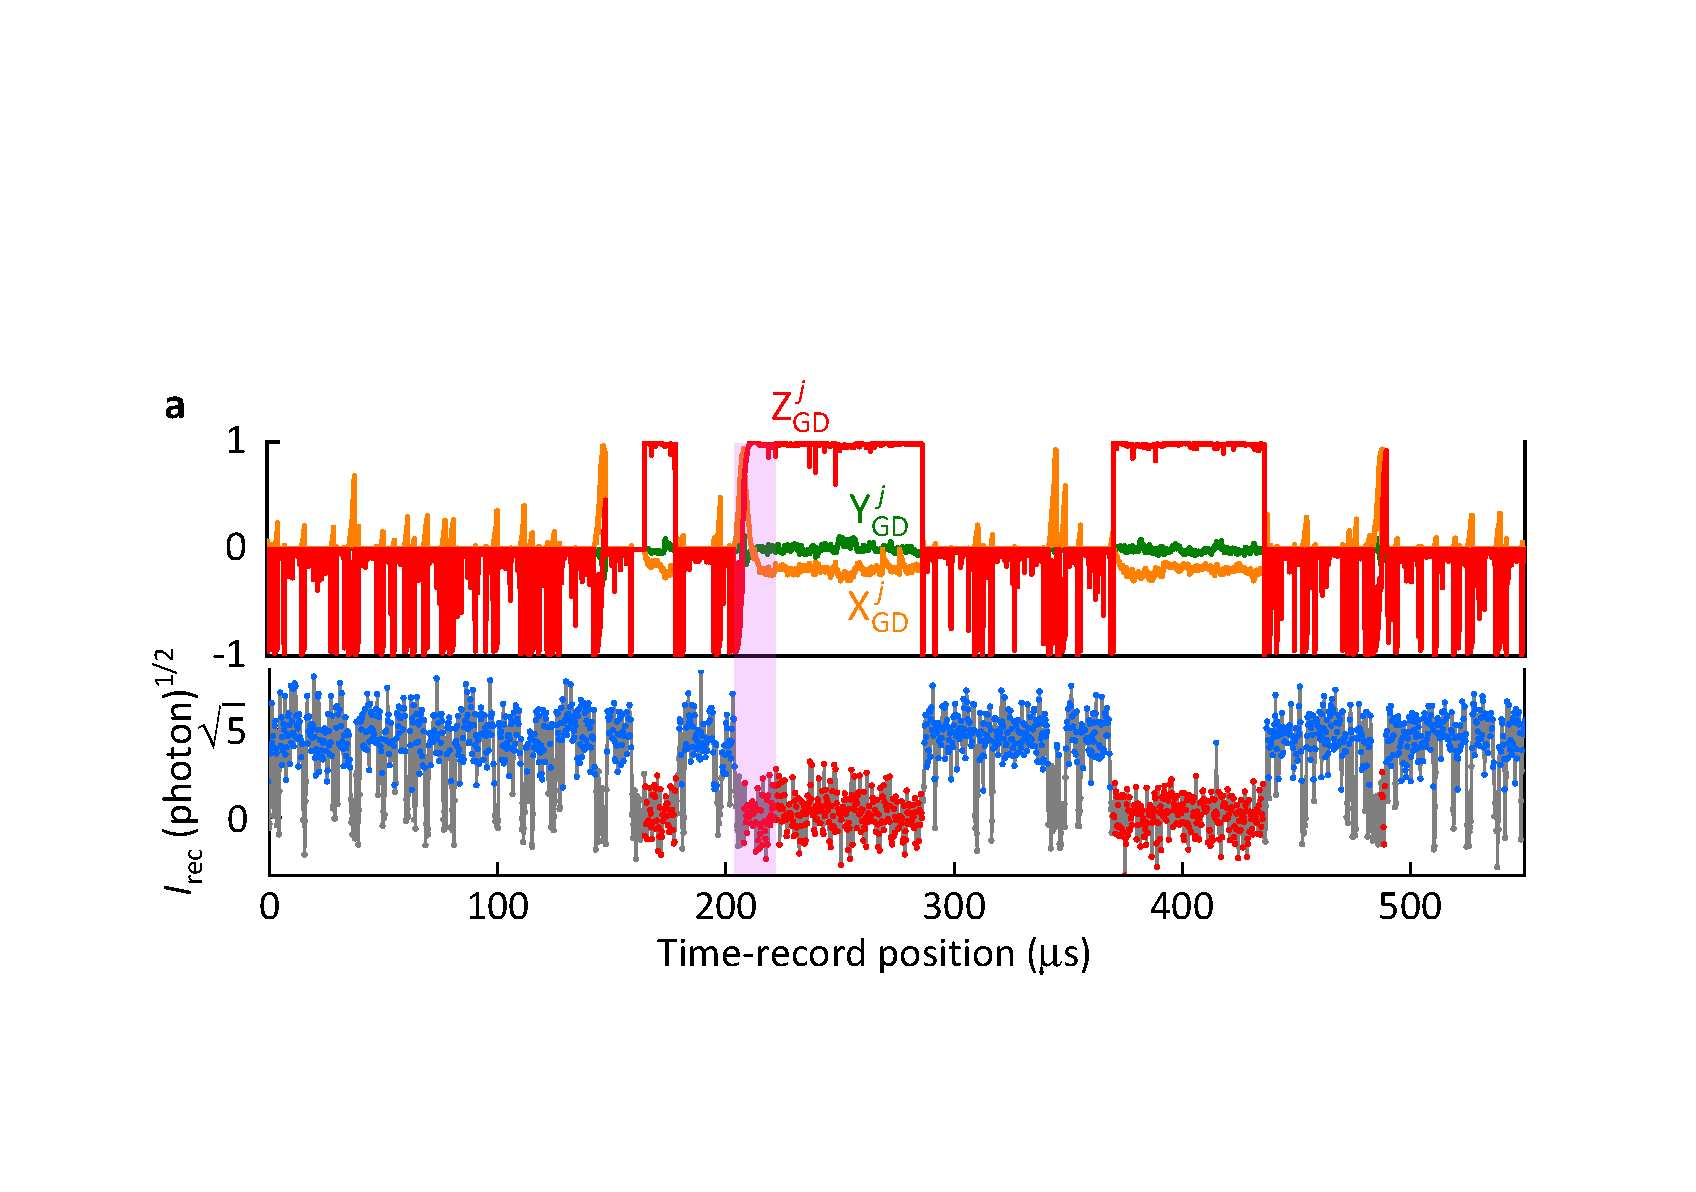
\includegraphics[width=11cm]{figure3.pdf}\raise0.0cm\hbox{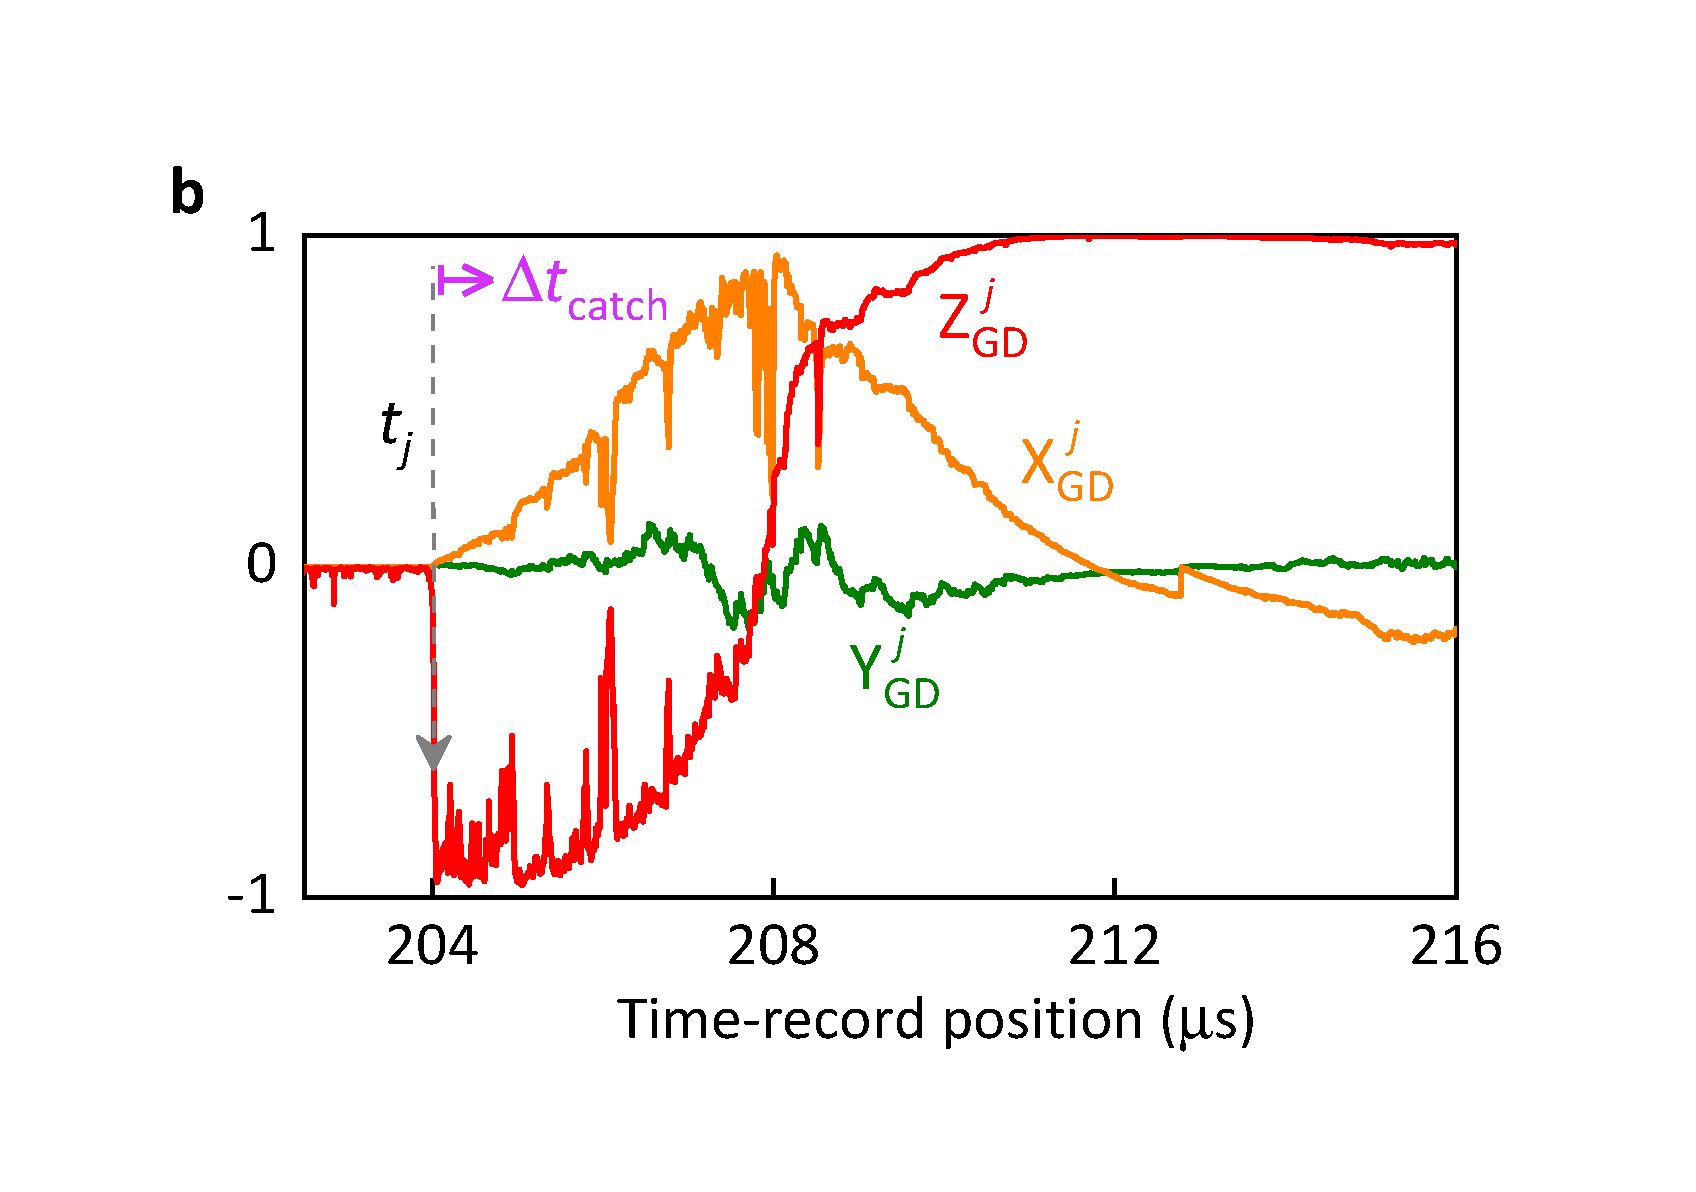
\includegraphics[width=7cm]{figure4.pdf}}
\caption{\label{fig:monte-carlo}
\textbf{Sampling of the Monte-Carlo simulation.} \textbf{a,} Simulated measurement quadrature $I_{\rm rec}$ and correlated trajectory computed from Eqs. (\ref{eqn:correlated_Z_GD}) and (\ref{eqn:correlated_X_GD&Y_GD}). Three sample intervals are shown. The earliest corresponds to leakage from the GBD-manifold, where a jump from $|{\rm G}\rangle$ to $|{\rm F}\rangle$ is followed by a jump from $|{\rm F}\rangle$ to $|{\rm D}\rangle$. The second and third sample intervals correspond to direct transitions from $|{\rm G}\rangle$ to $|{\rm D}\rangle$, which are continuously monitored and the object of the experiment. \textbf{b,} Expanded view of the shaded region of the second sample interval in panel (a). The evolution is continuous but not smooth, due to backaction noise from the continuously monitored readout. This feature is in sharp contrast to the perfect ``no-click'' readout upon which the simple theory of Sec.~\ref{sec:fluorescence_monitored_by_photon_counts} is based.
}
\vskip2.0cm

\hskip-1.75cm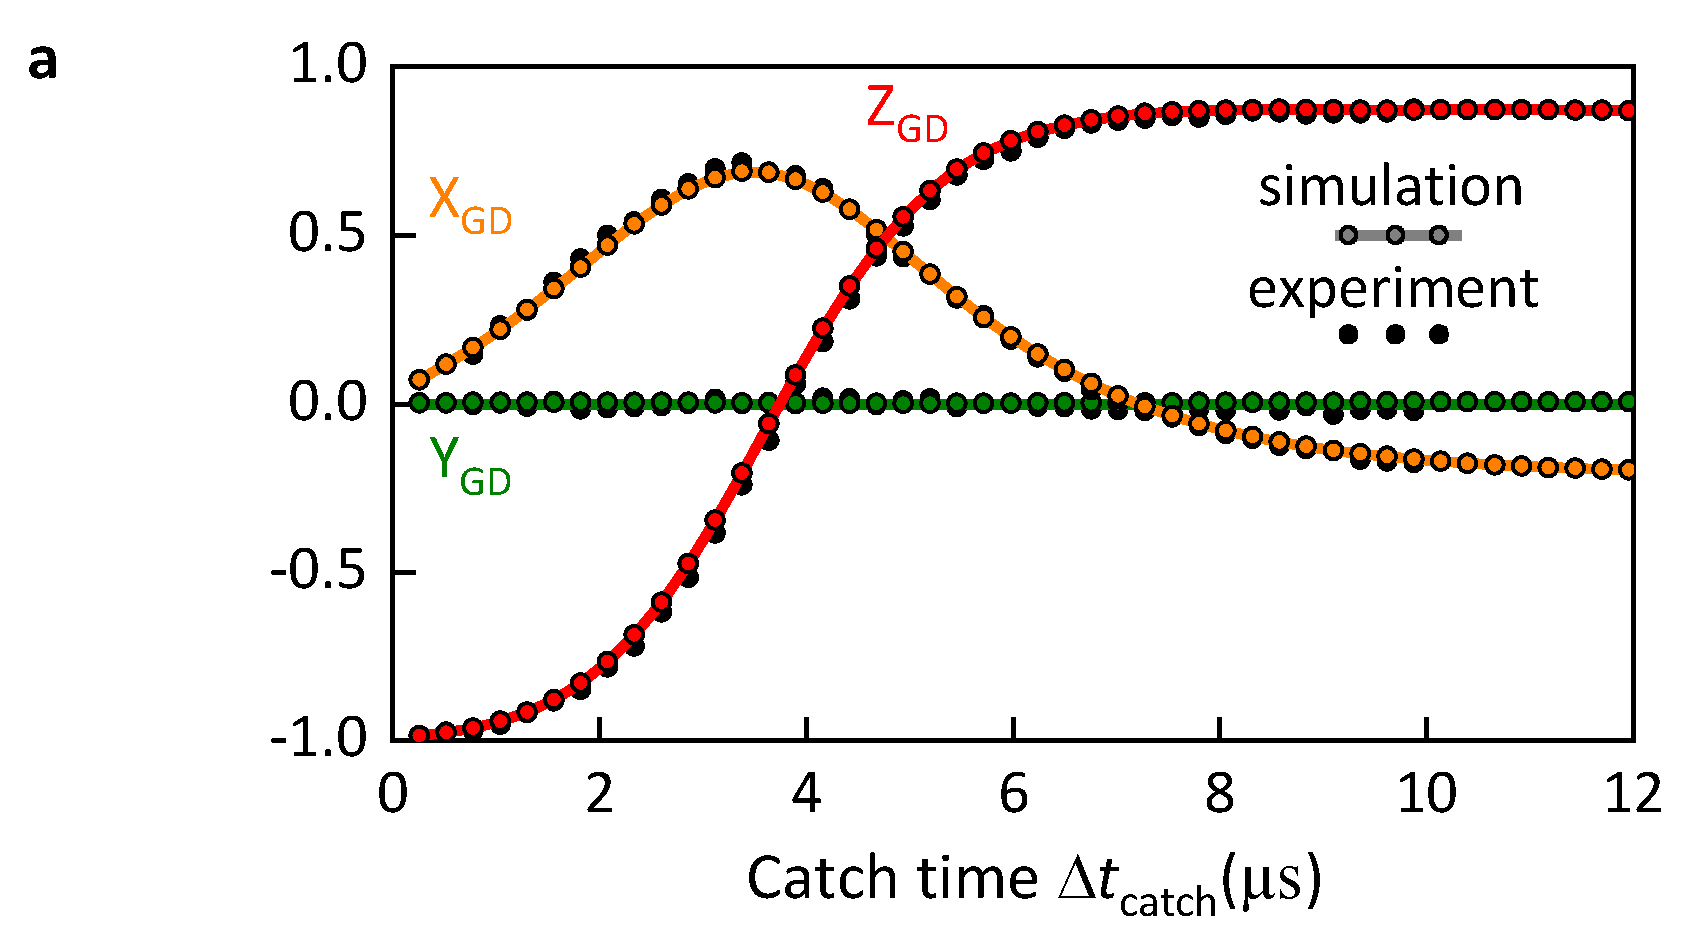
\includegraphics[width=9cm]{figure1.pdf}\hskip1cm
\vskip0.5cm
\hskip-1.75cm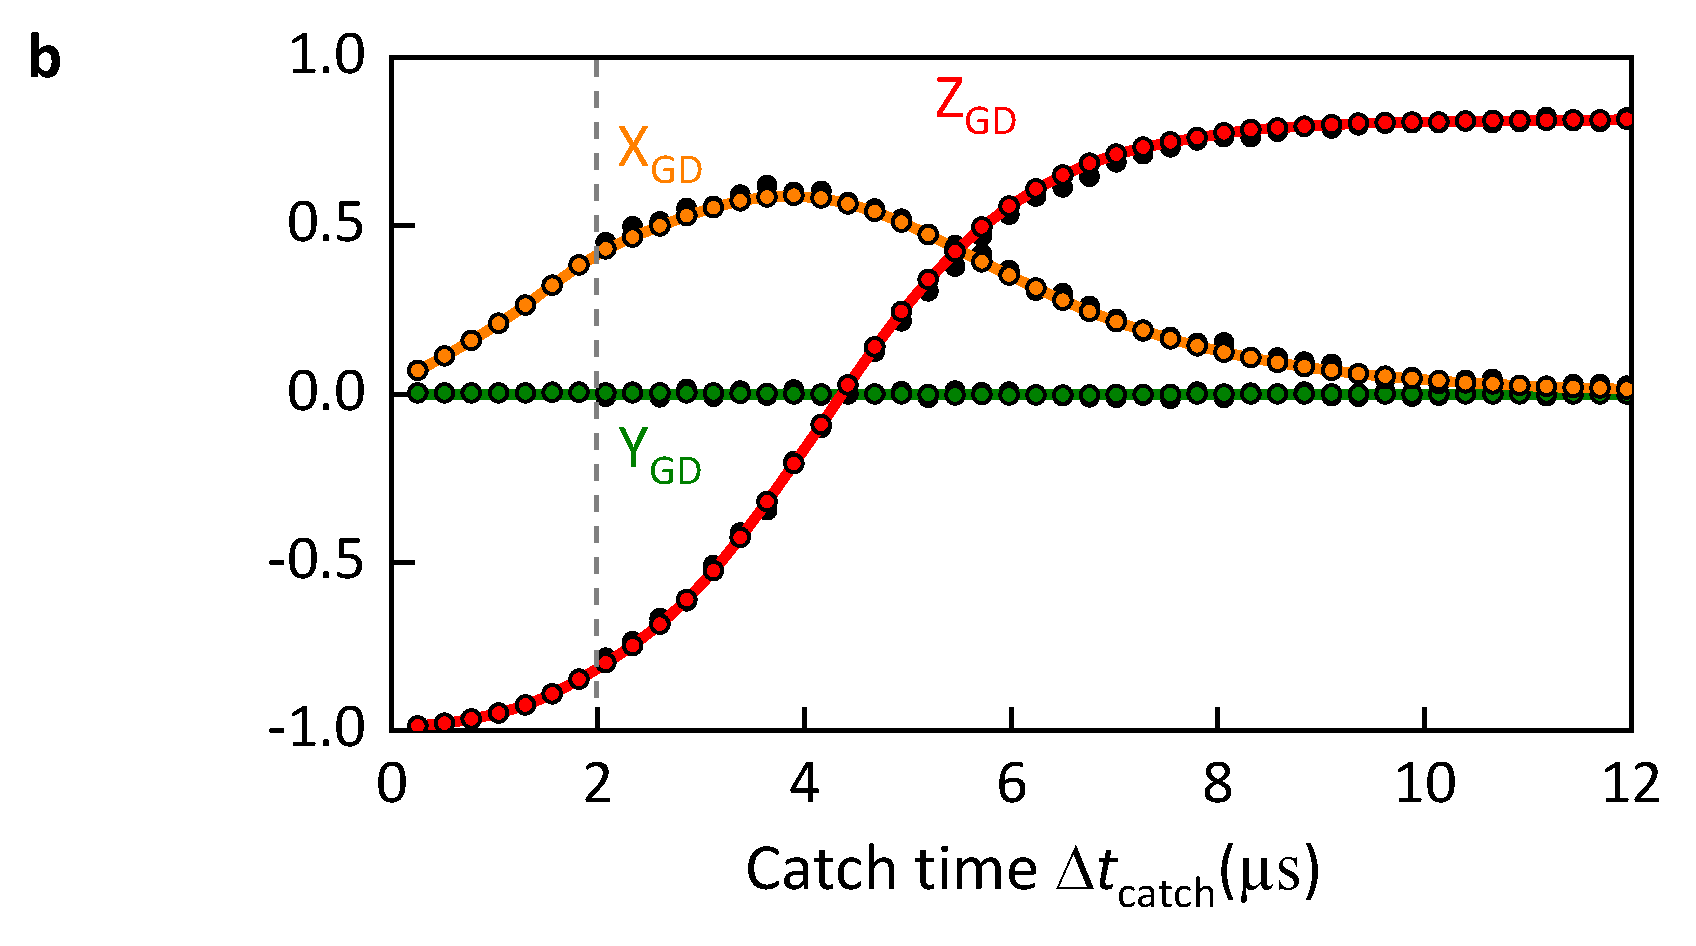
\includegraphics[width=9cm]{figure2.pdf}
\caption{\label{fig:simulation_vs_experiment}
\textbf{Comparison between simulation and experiment.} 
\textbf{a,}
 Simulated data set obtained with Rabi drive $\Omega_{\rm DG}$ turned on for the entire $\Delta t_{\rm catch}$; parameters taken from Table~\ref{table:table2} and leakage from the GBD-manifold included with $(\gamma_{\rm FG},\gamma_{\rm FD})/2\pi=0.38\mkern2mu{\rm kHz}$ and $(\gamma_{\rm GF},\gamma_{\rm DF})/2\pi=11.24\mkern2mu{\rm kHz}$. \textbf{b,} 
Simulated data set obtained with Rabi drive $\Omega_{\rm DG}$ turned off at time $\Delta t_{\rm on}=2\mkern2mu\mu{\rm s}$; parameters taken from Table \ref{table:table2} and leakage from the GBD-manifold included with $\gamma_{\rm FG}/2\pi=0.217\mkern2mu{\rm kHz}$, $\gamma_{\rm FD}/2\pi=4.34\mkern2mu{\rm kHz}$, $\gamma_{\rm GF}/2\pi=11.08\mkern2mu{\rm kHz}$, and $\gamma_{\rm DF}/2\pi=15.88\mkern2mu{\rm kHz}$. When leakage from the GBD-manifold is omitted, the ${\rm Z}_{\rm GD}$ curve rises more sharply and settles to a value that is  10\% (20\%) higher in panel (a) (panel (b)).
}
\end{centering}
\end{figure}





\subsection{Error budget}
\label{sec:Error-budget}

\subsubsection{Imperfections}
Various imperfections are expected to reduce the maximum coherence recovered in the measurement of ${\rm X}_{\rm GD}(\Delta t_{\rm catch})$. They include: \begin{enumerate}[(i)]
\item Readout errors when inferring $|{\rm B}\rangle$ to not-$|{\rm B}\rangle$ transitions and the reverse. Such errors affect the assignment of $\Delta t_{\rm catch}$, which can be either too short or too long to correlate correctly with the true state of the system.
\item Leaks from the GBD-manifold to higher excited states. These errors mimic a $|{\rm B}\rangle$ to not-$|{\rm B}\rangle$ transition, as in the first sample interval of Fig.~\ref{fig:monte-carlo}, yet the anticipated coherent evolution within the GBD-manifold does not occur.
\item Thermal jumps from $|{\rm G}\rangle$ to $|{\rm D}\rangle$. Such incoherent transitions contribute in a similar way to ${\rm Z}_{\rm GD}(\Delta t_{\rm catch})$, while making no contribution to the measured coherence.
\item Direct dephasing of the DG-coherence.
\item Partial distinguishability of $|{\rm G}\rangle$ and $|{\rm D}\rangle$. The readout cavity is not entirely empty of photons when the state is not-$|{\rm B}\rangle$, in which case the cross-Kerr interaction $\chi_{\rm D}|{\rm D}\rangle\langle{\rm D}|\hat c^\dagger\hat c$ shifts the $\Omega_{\rm DG}$ Rabi drive from resonance; hence, backaction noise is transferred from the photon number to ${\rm X_{\rm GD}}(\Delta t_{\rm catch})$.
\end{enumerate}

\subsubsection{Budget for lost coherence}
\label{sec:Budget-coherence}
The maximum coherence reported in the experiment is $0.71\pm0.005$. In the simulation it is a little lower at 0.69. By removing the imperfections from the simulation, one by one, we can assign a fraction of the total coherence loss to each. Readout errors are eliminated by identifying transitions between $|{\rm B}\rangle$ and not-$|{\rm B}\rangle$ in the ket $|\psi\rangle$ rather than from the simulated measurement record; all other imperfections are turned off by setting some parameter to zero. The largest coherence loss comes from readout errors, whose elimination raises the ${\rm X}_{\rm GD}(\Delta t_{\rm catch})$ maximum by 0.09. The next largest comes from leakage to higher excited states, which raises the maximum by a further 0.06. Setting $\chi_{\rm D}$ to zero adds a further 0.04, and thermal transitions and pure dephasing together add 0.02. Figure \ref{fig:coherence_loss} illustrates the change in the distribution of ${\rm X}_{\rm GD}^j(\Delta t_{\rm catch})$ samples underlying the recovery of coherence. The removal of the finger pointing to the left in panel (a) is mainly brought about by the elimination of readout errors, while the reduced line of zero coherence marks the elimination of leakage to higher excited states. Aside from these two largest changes, there is also a sharpening of the distribution, at a given $\Delta t_{\rm catch}$, when moving from panel (a) to panel (b). Having addressed the five listed imperfections, a further 10\% loss remains unaccounted for, i.e., the distribution of panel (b) is not a line passing through ${\rm X}_{\rm GD}^j(\Delta t_{\rm mid})=1$. The final 10\% is explained by the heterodyne detection backaction noise,  a function of the drive and measurement parameters, displayed in panel (b) of Fig.~\ref{fig:monte-carlo}.








\begin{figure}[!ht]
\begin{centering}
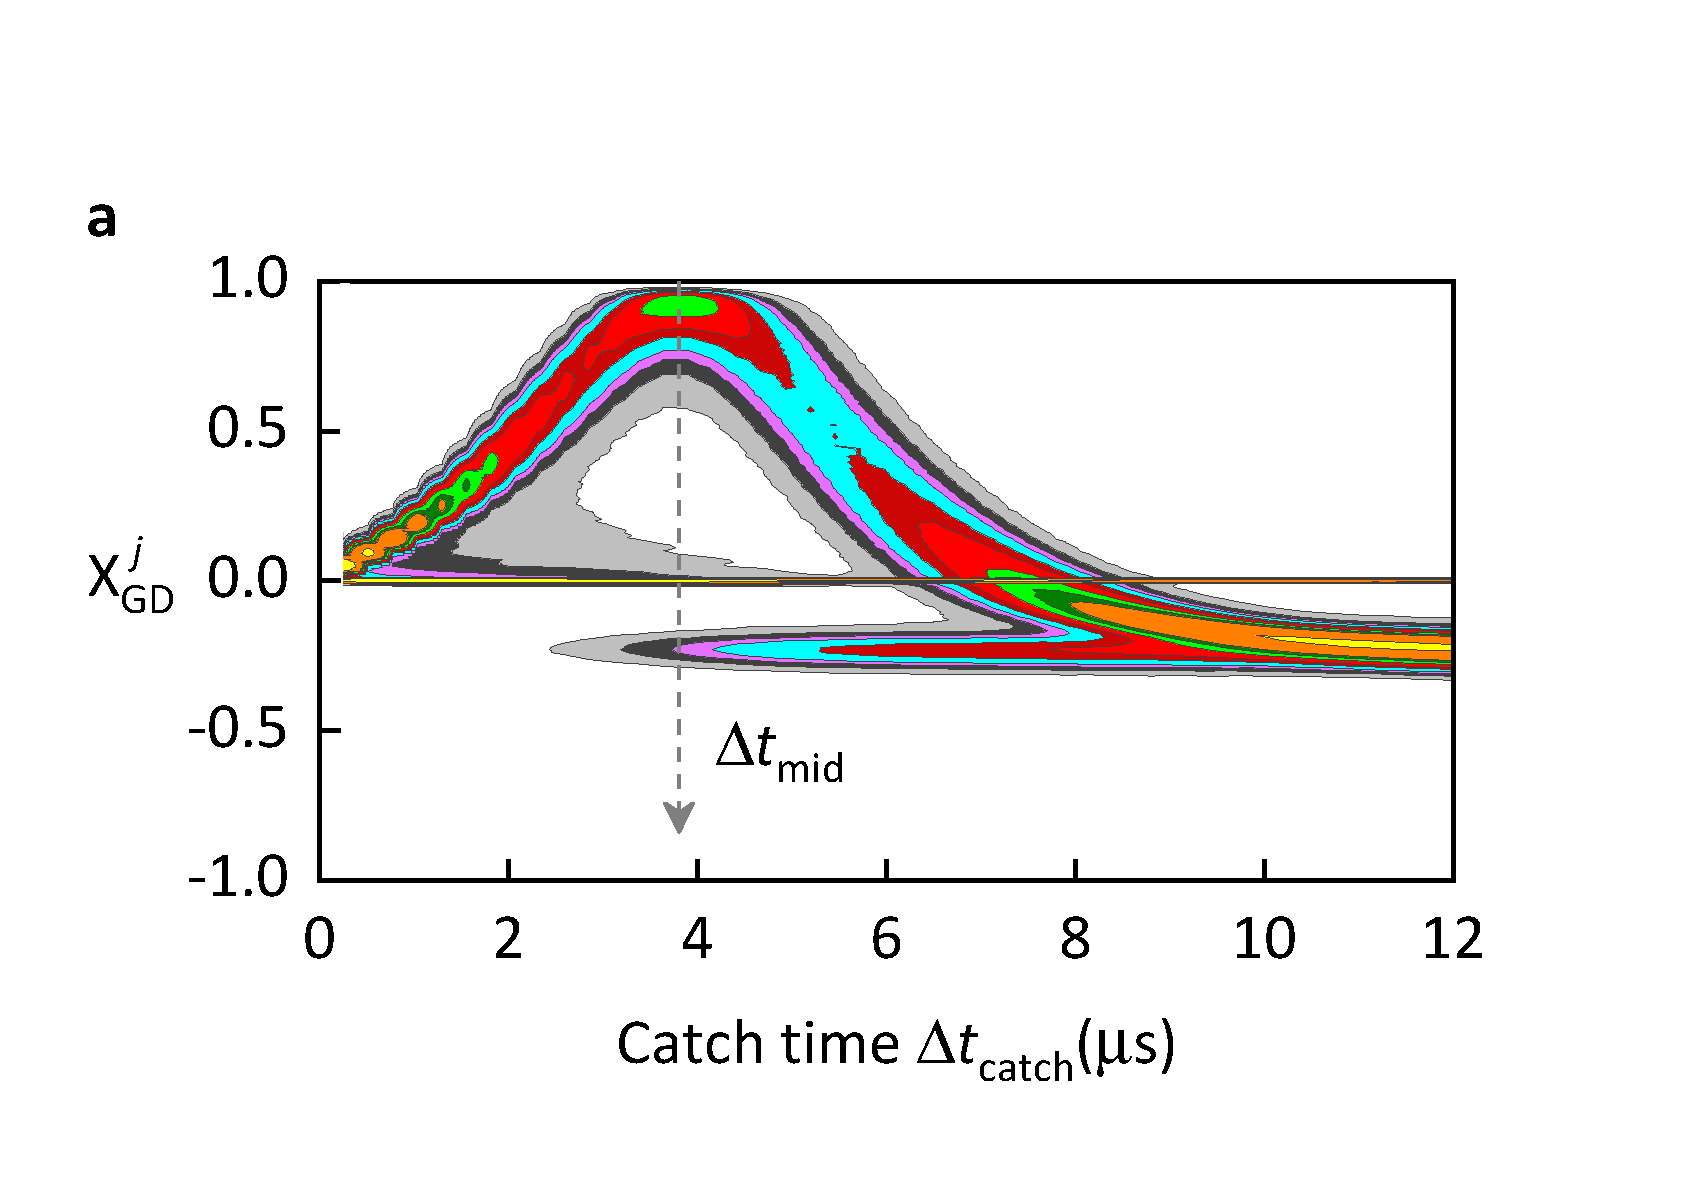
\includegraphics[height=4.8cm]{figure5.pdf}\hskip0.25cm\hbox{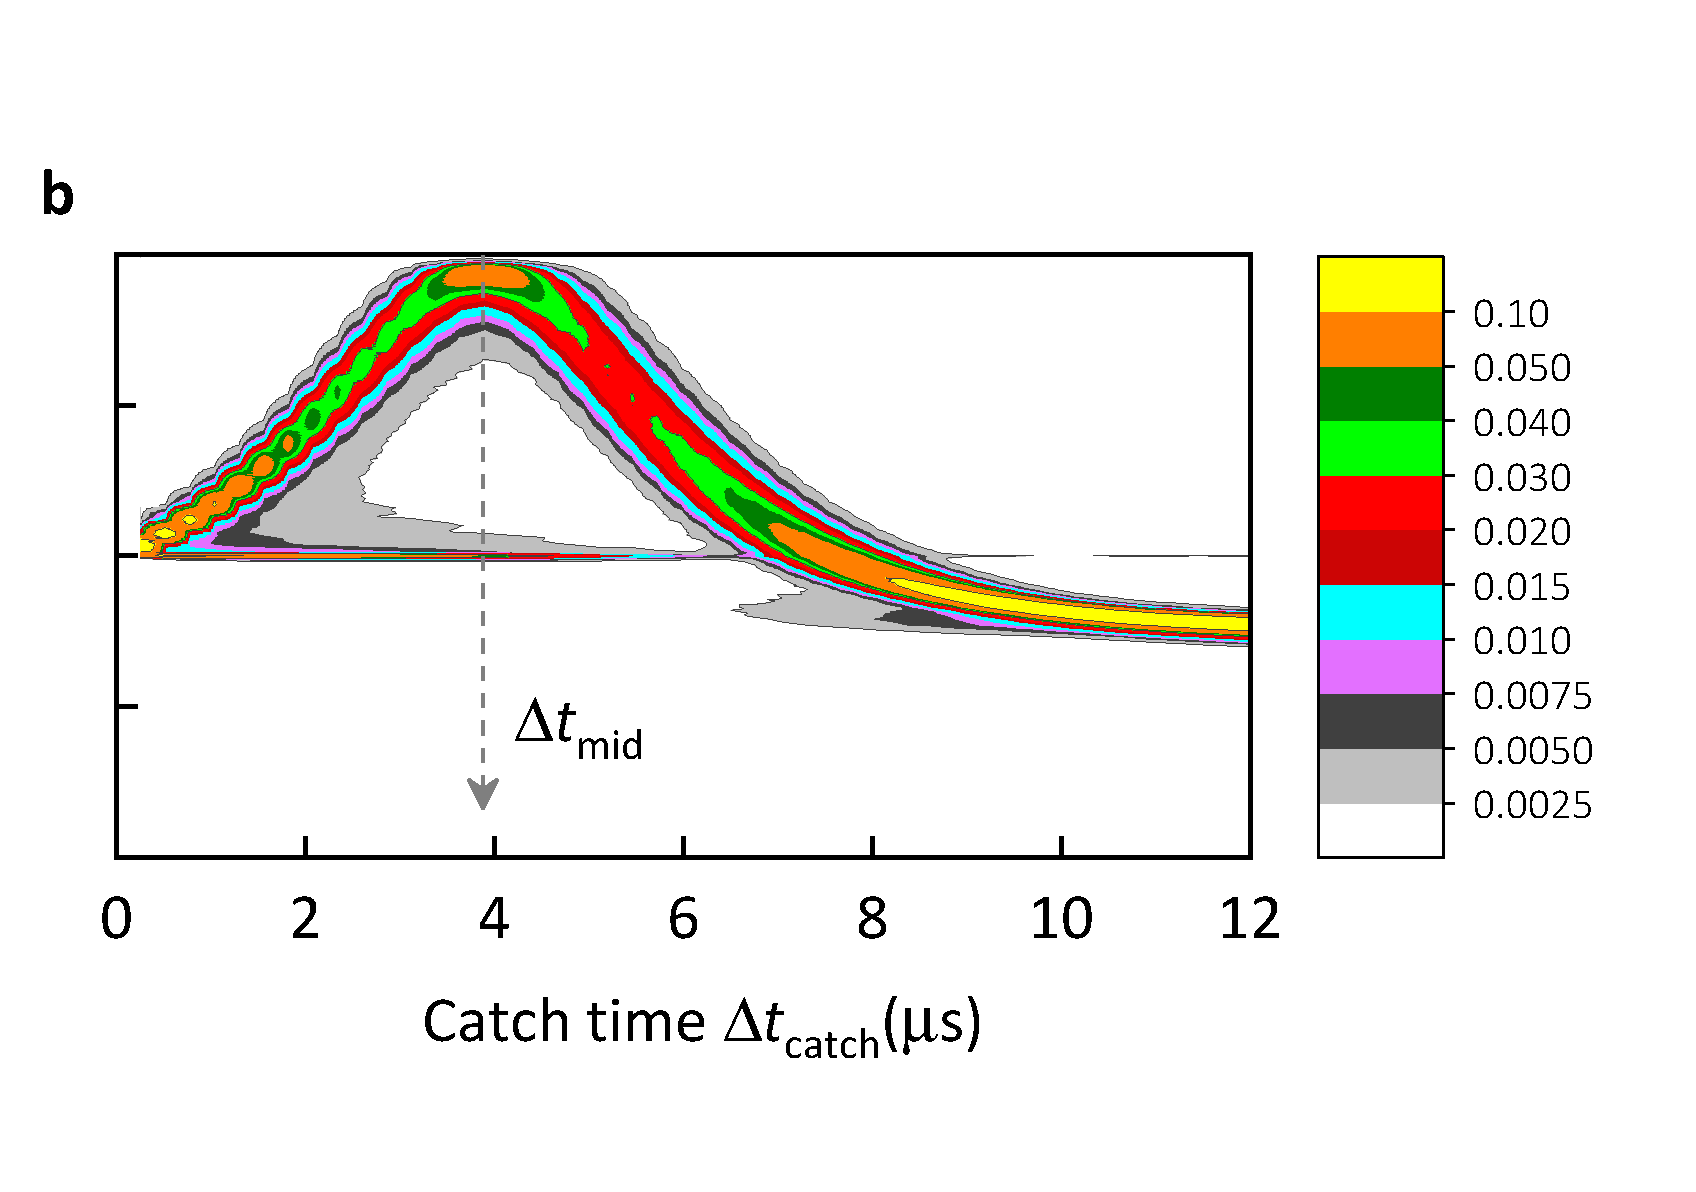
\includegraphics[height=4.8cm]{figure6.pdf}}
\caption{\label{fig:coherence_loss}
\textbf{Coherence loss through sample to sample fluctuations.} \textbf{a,} Contour plot of the distribution of ${\rm X}_{\rm GD}^j(\Delta t_{\rm catch})$ samples corresponding to the simulated data set displayed in panel (a) of Fig.~\ref{fig:simulation_vs_experiment}. \textbf{b,} Same as panel (a) but with transitions between $|{\rm B}\rangle$ and not-$|{\rm B}\rangle$ identified in the ket $|\psi\rangle$ rather than from the simulated measurement record, and with changed parameters: $(\gamma_{\rm FG},\gamma_{\rm FD},\gamma_{\rm GF},\gamma_{\rm DF})/2\pi=0$, $n_{\rm th}^{\rm B}=n_{\rm th}^{\rm D}=0$, $T_2^{\rm D}=2T_1^{\rm D}$, and $\chi_{\rm D}/2\pi=0$.
}
\end{centering}
\end{figure}

















\begin{table}
\begin{centering}
\begin{tabular}{>{\centering}p{0.5\textwidth}>{\centering}p{0.5\textwidth}}
     \textbf{(a)} In presence of $\Omega_{\mathrm{DG}}$  \\
 & \textbf{(b)} In absence of $\Omega_{\mathrm{DG}}$  \\
\tabularnewline
\centering{}\renewcommand*\arraystretch{1.2}
\begin{tabular}{cc|crcllrrlcr}
Parameter & \multicolumn{1}{c}{} &  & \multicolumn{3}{c}{Experiment} &  & \multicolumn{3}{c}{Simulation} &  & Error\tabularnewline
\hline 
\rule{0pt}{3ex} $a$ &  &  & -0.07 & $\pm$ & 0.005 &  & -0.07 & $\pm$ & 0.005 &  & 0.5\%\tabularnewline
$a'$ &  &  & -0.21 & $\pm$ & 0.005 &  & -0.22 & $\pm$ & 0.005 &  & 2\%\tabularnewline
$b$ &  &  & 0.94 & $\pm$ & 0.005 &  & 0.95 & $\pm$ & 0.005 &  & 1\%\tabularnewline
$b'$ &  &  & 0.93 & $\pm$ & 0.005 &  & 0.91 & $\pm$ & 0.005 &  & 2\%\tabularnewline
$c$ &  &  & -2.32 & $\pm$ & 0.03 &  & -2.27 & $\pm$ & 0.03 &  & 2\%\tabularnewline
$c'$ &  &  & -2.04 & $\pm$ & 0.03 &  & -2.05 & $\pm$ & 0.03 &  & 0.5\%\tabularnewline
$\tau$ &  &  & 1.64 & $\pm$ & 0.01 &  & 1.65 & $\pm$ & 0.01 &  & 0.5\%\tabularnewline
$\tau'$ &  &  & 1.74 & $\pm$ & 0.01 &  & 1.76 & $\pm$ & 0.01 &  & 1\%\tabularnewline
\end{tabular} & \centering{}\renewcommand*\arraystretch{1.2}
\begin{tabular}{cc|crcllrrlcr}
Parameter & \multicolumn{1}{c}{} &  & \multicolumn{3}{c}{Experiment} &  & \multicolumn{3}{c}{Simulation} &  & Error\tabularnewline
\hline 
\rule{0pt}{3ex} $a$ &  &  & -0.11 & $\pm$ & 0.005 &  & -0.10 & $\pm$ & 0.005 &  & 8\%\tabularnewline
$a'$ &  &  & 0 & $\pm$ & 0 &  & 0 & $\pm$ & 0 &  & 0\%\tabularnewline
$b$ &  &  & 0.92 & $\pm$ & 0.008 &  & 0.91 & $\pm$ & 0.008 &  & 1\%\tabularnewline
$b'$ &  &  & 0.61 & $\pm$ & 0.005 &  & 0.60 & $\pm$ & 0.005 &  & 2\%\tabularnewline
$c$ &  &  & -1.96 & $\pm$ & 0.05 &  & -2.10 & $\pm$ & 0.05 &  & 7\%\tabularnewline
$c'$ &  &  & -1.97 & $\pm$ & 0.05 &  & -2.05 & $\pm$ & 0.05 &  & 4\%\tabularnewline
$\tau$ &  &  & 2.17 & $\pm$ & 0.05 &  & 2.03 & $\pm$ & 0.05 &  & 6\%\tabularnewline
$\tau'$ &  &  & 1.98 & $\pm$ & 0.05 &  & 1.92 & $\pm$ & 0.05 &  & 3\%\tabularnewline
\end{tabular}\tabularnewline
\end{tabular}
\par\end{centering}
\caption{\label{tab:Comparison-of-parameters} \textbf{Comparison between 
parameters extracted from the simulation and those from the experiment}. 
\textbf{a,}
Parameters obtained from fits of the simulated and measured data for the catch protocol
in the presence of the Rabi drive $\Omega_{{\rm DG}}$ throughout the
entire duration of the quantum jump, data shown in Fig.~\ref{fig:simulation_vs_experiment}a. 
\textbf{b,} Parameters obtained
from fits of the simulated and measured data
for the catch protocol in the absence of the $\Omega_{{\rm DG}}$
during the flight of the quantum jump for $\Delta t_{\mathrm{on}}=2\mathrm{\ \mu s}$, data shown in  Fig.~\ref{fig:simulation_vs_experiment}b.
}
\end{table}











\subsection{Signal-to-noise ratio (SNR) and de-excitation measurement efficiency\label{subsec:Signal-to-noise-ratio-(SNR)}}

As discussed in the Methods section, the catch protocol hinges on
the efficient detection of de-excitations from $|{\rm B}\rangle$
to $|{\rm G}\rangle$. In atomic physics, de-excitations are typically
monitored by a \emph{direct} detection method, employing a photodetector.
Alternatively, de-excitations can be monitored by an\emph{ indirect}
method, as done in our experiment. In this subsection, we discuss
the efficiency of both methods. For the indirect method, using simple
analytics, we estimate the \emph{total} efficiency of time-continuous,
uninterrupted monitoring of de-excitations from $|{\rm B}\rangle$
to $|{\rm G}\rangle$ to be $\eta_{\mathrm{eff,clk}}=0.90\pm0.01$
for the parameters of our experiment, with integration time $T_{\mathrm{int}}=0.26\,\mathrm{\mu s}$.
The simple analysis of this section complements the numerical one
of the previous section, Sec.~\ref{sec:Budget-coherence}.

\emph{Direct monitoring method in atomic physics.} The direct method
monitors for a $|{\rm B}\rangle$ de-excitation by collecting and
absorbing the photon radiated in the de-excitation. The \emph{total}
measurement efficiency of this method is limited by i) collection
efficiency \textemdash{} the fraction of emitted photons collected
by the detector in its own input spatial modes (for instance, as determined
by the solid angle) \textemdash{} typically falls in the range 0.1
- 50\%,\cite{Volz2011} ii) the efficiency of detecting the absorption
of a single photon, which falls in the range 1 - 90\%,\cite{Eisaman2011}
and iii) non-idealities of the photodetector apparatus, including
its dead time, dark counts, jitter, etc.\cite{Eisaman2011} The combination
of these inefficiencies presents an almost insurmountable challenge
in experimental atomic physics for realizing continuous, time-resolved
detection of nearly every single photon emitted by the three-level
atom, required to faithfully catch the jump. 

\emph{Direct monitoring method with superconducting circuits.} While
technologically very different, the direct monitoring method with
superconducting circuits is conceptually similar to atomic method
but can readily achieve high collection efficiencies.\cite{Katz2008,Vijay2011,Riste2012-qubit-measure-reset,Vijay2012,Hatridge2013,Murch2013a,deLange2014,Roch2014,Weber2014,Campagne-Ibarcq2014,Macklin2015,Campagne2016-Fluorescence,Campagne-Ibarcq2016,Hacohen-Gourgy2016-non-comm,Naghiloo2016,White2016,Ficheux2017,Naghiloo2017-thermo,Tan2017,Hacohen-Gourgy2018,Heinsoo2018,Bultink2018}
 However, the energy of the emitted microwave photon is exceedingly
small \textemdash{} $23\text{ }\mathrm{\mu eV}$, about a part per
100,000 of the energy of a single optical photon \textemdash{} which
essentially forbids the direct detection of the photon with near-unit
efficiency. This is because the propagating photon is unavoidably
subjected to significant loss, added spurious noise, amplifier non-idealities,
etc. In our experiment, these imperfections reduce the full measurement/amplification
chain efficiency from its ideal value\cite{Hatridge2013,Macklin2015,Bultink2018}
of 1 to a modest $\eta=0.33\pm0.03$, corresponding to the direct
detection of approximately only one out of every three single photons
\textemdash{} insufficient for the catch protocol.

\subsubsection{Indirect monitoring method with superconducting circuits}

Alternatively, the indirect monitoring method couples the atom to
an ancillary degree of freedom, which is itself monitored in place
of the atom. In our experiment, the atom is strongly, dispersively
coupled to the ancillary readout cavity. The cavity scatters a probe
tone, whose phase shift constitutes the readout signal, as discussed
in the Methods section. Since the probe tone can carry itself many
photons, this scheme increases the signal-to-noise ratio ($\mathrm{SNR}$)
and, hence, the total efficiency ($\eta_{\mathrm{eff,clk}}$) of detecting
a $|{\rm B}\rangle$ de-excitation. Note that the efficiency $\eta_{\mathrm{eff,clk}}$
should not be confused with the efficiency of a photodetector or the
efficiency $\eta$ of the measurement/amplification chain, since $\eta_{\mathrm{eff,clk}}$
includes the effect of all readout imperfections and non-idealities,
state discrimination and assignment errors, etc. see below. In the
remainder of this section, we estimate the SNR and efficiency $\eta_{\mathrm{eff,clk}}$
of the experiment.

\emph{SNR of the indirect (dispersive) method.}  The output of the
measurement and amplification chain monitoring the readout cavity
is proportional to the complex heterodyne measurement record $\zeta\left(t\right)$,
which obeys the It\^{o} stochastic differential equation, see Eq.~\eqref{eq:heterodyne-current},\footnote{Since the bandwidth of the measurement chain, $\kappa_{\mathrm{filter}}$,
is significantly larger than that, $\kappa$, of the readout cavity,
$\kappa_{\mathrm{filter}}\gg\kappa$, we can neglect the effect of
$\kappa_{\mathrm{filter}}$ for simplicity of discussion, see Eqs.~\eqref{eq:dI_rec}
and~\eqref{eq:dQ_rec}. } 
\begin{equation}
\mathrm{d}\zeta\left(t\right)=\sqrt{\eta\kappa}\frac{\langle\psi\left(t\right)|\hat{a}|\psi\left(t\right)\rangle}{\langle\psi\left(t\right)|\psi\left(t\right)\rangle}\mathrm{d}t+\mathrm{d}Z\left(t\right),\label{eq:heterodyne-current2}
\end{equation}
where $\hat{a}$ is the cavity amplitude operator in the Schr\"{o}dinger
picture, $\eta$ is the total measurement efficiency of the amplification
chain \textemdash{} again, not to be confused with the de-excitation
measurement efficiency, $\eta_{\mathrm{eff,clk}}$ \textemdash{} and
$\mathrm{d}Z$ is the complex Wiener process increment, defined below
Eq.~\eqref{eq:heterodyne-current2}. A somewhat counterintuitive
property of Eq.~\eqref{eq:heterodyne-current2} is that  the heterodyne
record increment $\mathrm{d}\zeta\left(t\right)$ is stochastic and
noisy even when $\eta=1$, the case of ideal measurement in which
no signal is lost \textemdash{} the stochastic term, $\mathrm{d}Z$,
represents pure quantum vacuum fluctuations, which are inherent in
the case of heterodyne detection.\cite{Carmichael1993,Plenio1998,wiseman2010book}
Due to the unavoidable presence of these fluctuations, only an infinitesimal
amount of information about the system can be extracted from $\mathrm{d}\zeta$
at an instant of time. Finite amount of information is extracted by
integrating $\mathrm{d}\zeta$ for a finite duration $T_{\mathrm{int}}$,
\begin{equation}
s\equiv I_{\mathrm{rec}}+iQ_{\mathrm{rec}}\equiv\int_{0}^{T_{\mathrm{int}}}\mathrm{d}\zeta\left(t\right)\,,\label{eq:s=00003D}
\end{equation}
where $I_{\mathrm{rec}}$ and $Q_{\mathrm{rec}}$ are the in- and
out-of-phase quadrature components of one segment of the record. What
does $s$ correspond to? Its value depends on $\mathrm{d}\zeta$,
which depends on the state of the cavity, $|\psi\rangle$, which itself
depends on the occupation of $\ket{\mathrm{B}}$ \textemdash{} and
therefore $s$ contains the occupation of $\ket{\mathrm{B}}$. A de-excitation
of $\ket{\mathrm{B}}$ to $\ket{\mathrm{G}}$ can thus be detected
by monitoring $s$, whose value is different for the two states, since
the cavity is generally in the coherent state $\ket{\alpha_{\mathrm{B}}}$
or $\ket{\alpha_{\mathrm{G}}}$ when the atom is in $\ket{\mathrm{B}}$
or $\ket{\mathrm{G}}$, respectively. For the moment, assuming the
atom and cavity do not change states during the course of the measurement
duration $T_{\mathrm{int}}$, the stochastic integral in Eq.~\eqref{eq:s=00003D}
explicitly evaluates to 
\begin{equation}
s_{\mathrm{B,G}}=\left\{ \sqrt{\eta\kappa}\mathrm{Re}\left[\alpha_{\mathrm{B,G}}\right]T_{\mathrm{int}}+\frac{1}{\sqrt{2}}W_{I}\left(T_{\mathrm{int}}\right)\right\} +i\left\{ -\sqrt{\eta\kappa}\mathrm{Im}\left[\alpha_{\mathrm{B,G}}\right]T_{\mathrm{int}}+\frac{1}{\sqrt{2}}W_{Q}\left(T_{\mathrm{int}}\right)\right\} \,,\label{eq:s=00003DExplicit}
\end{equation}
where $W_{I,Q}$ denote independent Wiener processes, obeying the
conventional rules, $\mathrm{E}\left[W\left(t\right)\right]=0$ and
$\mathrm{Var}\left[W\left(t\right)\right]=t^{2}$. Equation~\eqref{eq:s=00003DExplicit}
shows that the distribution of the stochastic variable $s$ is a Gaussian
blob in the IQ plane centered at $\bar{s}_{\mathrm{B,G}}\equiv\operatorname{E}\left[s_{\mathrm{B,G}}\right]=\sqrt{\eta\gamma}T_{\mathrm{int}}\alpha_{\mathrm{B,G}}$
with width determined by the variance $\sigma_{\mathrm{B,G}}^{2}\equiv\operatorname{Var}\left[s_{\mathrm{B,G}}\right]=\frac{1}{2}T_{\mathrm{int}}$.
We can thus define the SNR of the experiment by comparing the distance
between the two pointer distributions to their width, 
\begin{equation}
\mathrm{SNR}\equiv\left|\frac{\bar{s}_{\mathrm{B}}-\bar{s}_{\mathrm{G}}}{\sigma_{\mathrm{B}}+\sigma_{\mathrm{G}}}\right|^{2}\,,\label{eq:SNR-defn}
\end{equation}
where the B (resp., G) subscript denotes signals conditioned on the
atom being in $\ket{\mathrm{B}}$ (resp., $\ket{\mathrm{G}}$). In
terms of $\ket{\alpha_{\mathrm{B}}}$ and $\ket{\alpha_{\mathrm{G}}}$,
\begin{equation}
\mathrm{SNR}=\frac{1}{2}\eta\kappa T_{\mathrm{int}}\left|\alpha_{\mathrm{B}}-\alpha_{\mathrm{G}}\right|^{2}\,,
\end{equation}
which can be expressed in terms of the parameters of the experiment,
summarized in Table~\ref{tab:system-params},
\begin{equation}
\mathrm{SNR}=\frac{1}{2}\eta\kappa T_{\mathrm{int}}\left[\cos\left(\arctan\left(\frac{\kappa}{2\chi_{\mathrm{BG}}}\right)\right)\right]^{2}\bar{n}\,,\label{eq:SNR-expression}
\end{equation}
Holding other parameters fixed, according to Eq.~\eqref{eq:SNR-expression},
the SNR can be increased arbitrarily by increasing $\bar{n}$, which
can be readily done by increasing the amplitude of the cavity probe
tone. A higher SNR for $s$ corresponds to a higher SNR for measuring
an atom de-excitation, since $s$ is a proxy of the $\ket{\mathrm{B}}$
population. Thus, the indirect cavity monitoring can overcome the
typical degradation in SNR imposed by the inefficiencies and non-idealities
of the measurement chain, $\eta$. In practice, the SNR increase
with $\bar{n}$ is bounded from above, since with sufficiently high
$\bar{n}$ spurious non-linear effects become significant\cite{Boissonneault2008,Boissonneault2009-Photon-induced-relax,Minev2013,Sank2016-T1vsNbar,Khezri2016,Bultink2016,Khezri2017,Walter2017,Lescanne2018,Verney2018,Serniak2018}.
The cavity and non-linear coupling to the atom serve in effect as
a rudimentary embedded pre-amplifier at the site of the atom, which
transduces with amplification the de-excitation signal before its
SNR is degraded during propagation and further processing.

\emph{Discrimination efficiency of the indirect method.} While the
SNR provides a basic characterization of the measurement, it is useful
to convert it to a number between 0 and 1, which is called the discrimination
efficiency, $\eta_{\mathrm{disc}}$. It quantifies the degree to which
the two Gaussian distributions of $s$ are distinguishable,\cite{Gambetta2007-ProtocolsMsr}
\begin{equation}
\eta_{\mathrm{disc}}=\frac{1}{2}\operatorname{erfc}\left[-\sqrt{\frac{\mathrm{SNR}}{2}}\right]\,,\label{eq:eta-msr}
\end{equation}
where $\operatorname{erfc}$ denotes the complementary error function.
Equation~\eqref{eq:eta-msr} shows that increasing the SNR by separating
the $s_{\mathrm{B}}$ and $s_{\mathrm{G}}$ distributions far beyond
their spread, $\sigma_{\mathrm{B/G}}$, provides only marginal gain
as $\eta_{\mathrm{disc}}$ saturates to 1. Next, we calculate the
SNR and $\eta_{\mathrm{disc}}$ for the parameters of the experiment
and discuss corrections due to readout non-idealities. 

\emph{A first comparison to the experiment. }A first estimate of the
SNR and $\eta_{\mathrm{disc}}$ of the experiment are provided by
Eqs.~\eqref{eq:SNR-expression} and~\eqref{eq:eta-msr}. Using the
parameters of the experiment, summarized in Table~\ref{tab:system-params},
from these two equations, we find $\mathrm{SNR}=4.3\pm0.6$ and $\eta_{\mathrm{disc}}=0.98\pm0.007$.
Using data from the experiment, in particular, a second long IQ record
trace, represented by a short segment in Fig.~2a, we find the SNR
of the jumps experiment, by fitting the histogram of the trace with
a bi-Gaussian distribution, to be $\mathrm{SNR}=3.8\pm0.4$, corresponding
to $\eta_{\mathrm{\mathrm{disc}}}=0.96\pm0.01$. The measured values
are slightly lower than the analytics predict due to readout imperfections
not included in the calculation so far, such as state transitions
during $T_{\mathrm{int}}$, cavity transient dynamics, additional
pointer-state distributions, etc.

\emph{Effective click detection efficiency. }The dominant next-order
error is due to atom state transitions during the measurement window,
$T_{\mathrm{int}}$, which contributes an assignment error of approximately
$1-\eta_{\mathrm{asg}}=1-\exp\left(T_{\mathrm{int}}/\tau_{\mathrm{B}}\right)=0.06\pm0.001$
to the detection of a $|\mathrm{B}\rangle$ de-excitation. Combining
$\eta_{\mathrm{disc}}$ with $\eta_{\mathrm{asg}}$, we obtain the
total efficiency for detecting $\ket{\mathrm{B}}$ de-excitations
$\eta_{\mathrm{eff,clk}}=\eta_{\mathrm{disc}}\eta_{\mathrm{asg}}=0.90\pm0.01$,
consistent with the total readout efficiency of $0.91$ that is independently
estimated using the trajectory numerics, see Sec.~\ref{sec:Budget-coherence}.





























\nocite{apsrev41Control}
\bibliographystyle{apsrev4-1}
\bibliography{mycontrol,biblio}


\end{document} 
